\begin{minipage}[t]{0.47\linewidth}\textbf{0000} \hfill \num{-68}\,\%\par 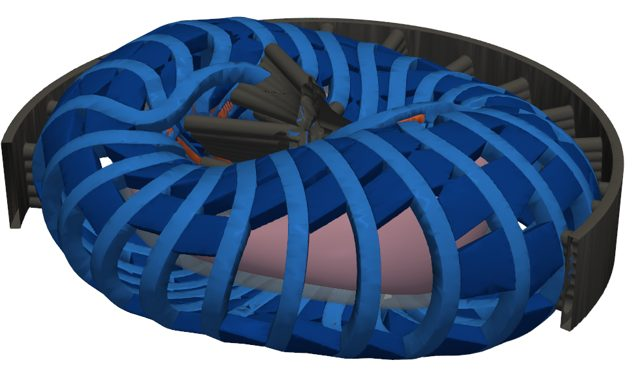
\includegraphics[width=\linewidth]{bilder/katalog/0000.jpg}\par\scriptsize \begin{tabular}{@{}l@{\,}r@{\quad}l@{\,}r@{}}Spulen & 24 & $\sigma_{99}$ & \num{840} MPa \\Verb./Paar & 10 & max. & \num{3425} MPa \\$E_V$ & \num{70} GPa & Dehnung & \num{0.42} \% \\Abstand & \num{0.18} & $B\cdot n$ & \num{1.98} ‰ \\Stahl & \num{23} kt & frei & \num{1.44} m \\\end{tabular}\par verletzt: Stahl σ99, Dehnung Wickelpaket. PicoGK: keine Überschneidung.\end{minipage}\hfill
\begin{minipage}[t]{0.47\linewidth}\textbf{0001} \hfill \num{-191}\,\%\par 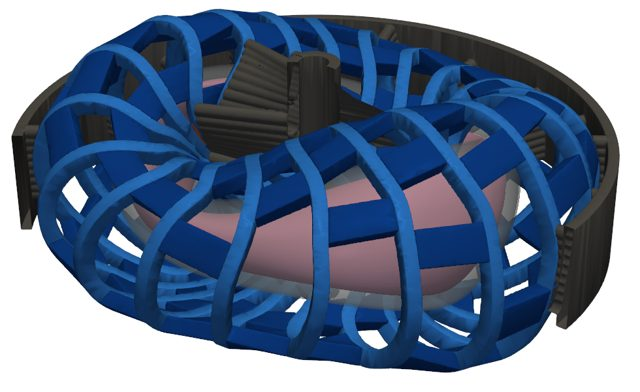
\includegraphics[width=\linewidth]{bilder/katalog/0001.jpg}\par\scriptsize \begin{tabular}{@{}l@{\,}r@{\quad}l@{\,}r@{}}Spulen & 20 & $\sigma_{99}$ & \num{1456} MPa \\Verb./Paar & 7 & max. & \num{3851} MPa \\$E_V$ & \num{135} GPa & Dehnung & \num{0.60} \% \\Abstand & \num{0.24} & $B\cdot n$ & \num{1.53} ‰ \\Stahl & \num{12} kt & frei & \num{2.00} m \\\end{tabular}\par verletzt: Stahl σ99, Dehnung Wickelpaket. PicoGK: keine Überschneidung.\end{minipage}\par\vspace{6pt}
\begin{minipage}[t]{0.47\linewidth}\textbf{0002} \hfill \num{-844}\,\%\par 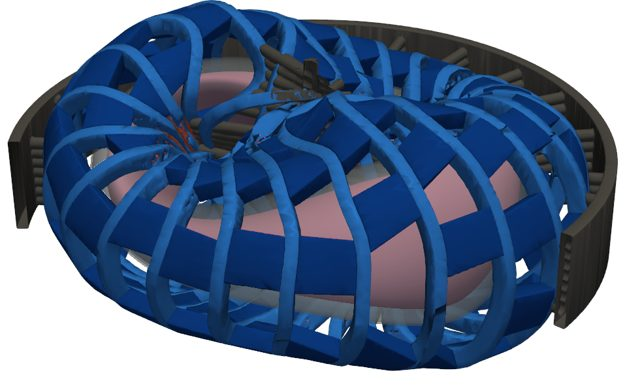
\includegraphics[width=\linewidth]{bilder/katalog/0002.jpg}\par\scriptsize \begin{tabular}{@{}l@{\,}r@{\quad}l@{\,}r@{}}Spulen & 24 & $\sigma_{99}$ & \num{4721} MPa \\Verb./Paar & 8 & max. & \num{13357} MPa \\$E_V$ & \num{25} GPa & Dehnung & \num{2.01} \% \\Abstand & \num{0.30} & $B\cdot n$ & \num{3.67} ‰ \\Stahl & \num{13} kt & frei & \num{2.39} m \\\end{tabular}\par verletzt: Stahl σ99, Dehnung Wickelpaket, Feldfehler B·n. PicoGK: keine Überschneidung.\end{minipage}\hfill
\begin{minipage}[t]{0.47\linewidth}\textbf{0003} \hfill \num{-216}\,\%\par 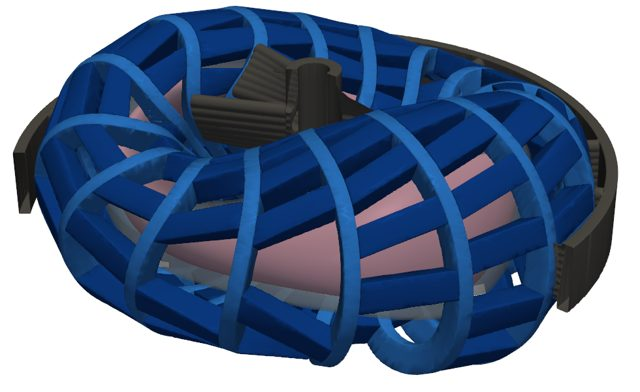
\includegraphics[width=\linewidth]{bilder/katalog/0003.jpg}\par\scriptsize \begin{tabular}{@{}l@{\,}r@{\quad}l@{\,}r@{}}Spulen & 16 & $\sigma_{99}$ & \num{617} MPa \\Verb./Paar & 12 & max. & \num{1361} MPa \\$E_V$ & \num{142} GPa & Dehnung & \num{0.26} \% \\Abstand & \num{0.20} & $B\cdot n$ & \num{9.48} ‰ \\Stahl & \num{20} kt & frei & \num{1.40} m \\\end{tabular}\par verletzt: Stahl σ99, Feldfehler B·n. PicoGK: keine Überschneidung.\end{minipage}\par\vspace{6pt}
\clearpage
\begin{minipage}[t]{0.47\linewidth}\textbf{0004} \hfill \num{-12}\,\%\par 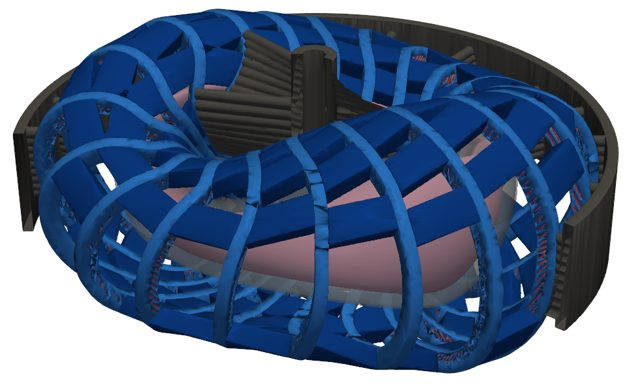
\includegraphics[width=\linewidth]{bilder/katalog/0004.jpg}\par\scriptsize \begin{tabular}{@{}l@{\,}r@{\quad}l@{\,}r@{}}Spulen & 20 & $\sigma_{99}$ & \num{558} MPa \\Verb./Paar & 10 & max. & \num{1085} MPa \\$E_V$ & \num{148} GPa & Dehnung & \num{0.26} \% \\Abstand & \num{0.19} & $B\cdot n$ & \num{1.81} ‰ \\Stahl & \num{19} kt & frei & \num{1.54} m \\\end{tabular}\par verletzt: Stahl σ99. PicoGK: keine Überschneidung.\end{minipage}\hfill
\begin{minipage}[t]{0.47\linewidth}\textbf{0005} \hfill \num{-69}\,\%\par 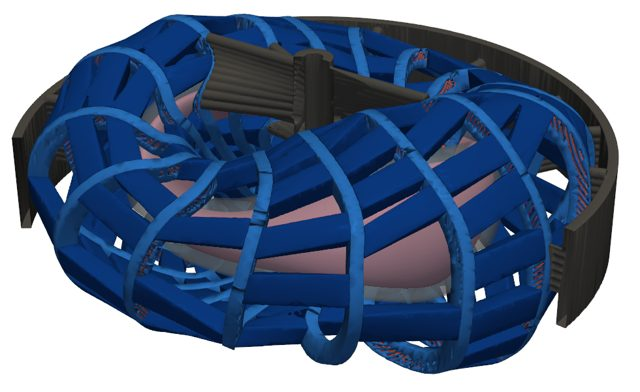
\includegraphics[width=\linewidth]{bilder/katalog/0005.jpg}\par\scriptsize \begin{tabular}{@{}l@{\,}r@{\quad}l@{\,}r@{}}Spulen & 16 & $\sigma_{99}$ & \num{844} MPa \\Verb./Paar & 13 & max. & \num{1847} MPa \\$E_V$ & \num{114} GPa & Dehnung & \num{0.35} \% \\Abstand & \num{0.15} & $B\cdot n$ & \num{2.40} ‰ \\Stahl & \num{23} kt & frei & \num{1.26} m \\\end{tabular}\par verletzt: Stahl σ99, Dehnung Wickelpaket, Neutronenfluenz. PicoGK: keine Überschneidung.\end{minipage}\par\vspace{6pt}
\begin{minipage}[t]{0.47\linewidth}\textbf{0006} \hfill \num{-1480}\,\%\par 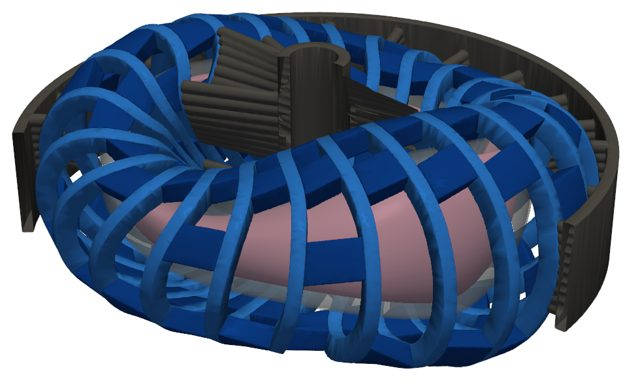
\includegraphics[width=\linewidth]{bilder/katalog/0006.jpg}\par\scriptsize \begin{tabular}{@{}l@{\,}r@{\quad}l@{\,}r@{}}Spulen & 24 & $\sigma_{99}$ & \num{536} MPa \\Verb./Paar & 6 & max. & \num{1222} MPa \\$E_V$ & \num{78} GPa & Dehnung & \num{0.22} \% \\Abstand & \num{0.12} & $B\cdot n$ & \num{1.77} ‰ \\Stahl & \num{14} kt & frei & \num{0.99} m \\\end{tabular}\par verletzt: Stahl σ99, Platz Package, Kernheizung, Neutronenfluenz. PicoGK: keine Überschneidung.\end{minipage}\hfill
\begin{minipage}[t]{0.47\linewidth}\textbf{0007} \hfill \num{-231}\,\%\par 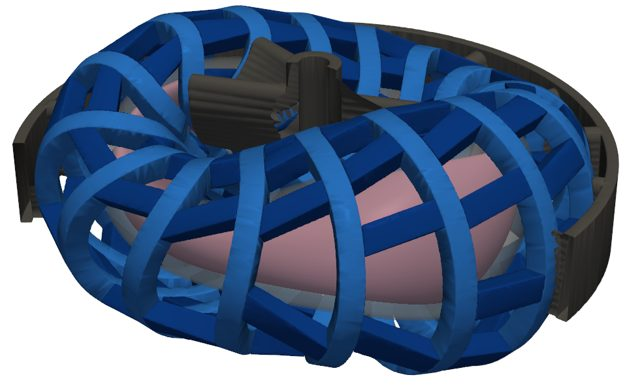
\includegraphics[width=\linewidth]{bilder/katalog/0007.jpg}\par\scriptsize \begin{tabular}{@{}l@{\,}r@{\quad}l@{\,}r@{}}Spulen & 16 & $\sigma_{99}$ & \num{870} MPa \\Verb./Paar & 8 & max. & \num{3574} MPa \\$E_V$ & \num{88} GPa & Dehnung & \num{0.42} \% \\Abstand & \num{0.16} & $B\cdot n$ & \num{9.92} ‰ \\Stahl & \num{17} kt & frei & \num{1.60} m \\\end{tabular}\par verletzt: Stahl σ99, Dehnung Wickelpaket, Feldfehler B·n. PicoGK: keine Überschneidung.\end{minipage}\par\vspace{6pt}
\clearpage
\begin{minipage}[t]{0.47\linewidth}\textbf{0008} \hfill \num{27}\,\%\par 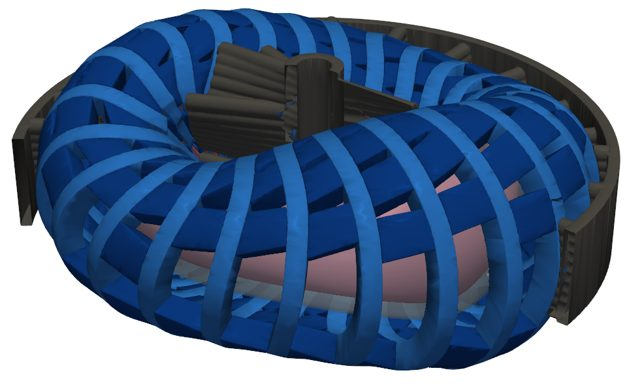
\includegraphics[width=\linewidth]{bilder/katalog/0008.jpg}\par\scriptsize \begin{tabular}{@{}l@{\,}r@{\quad}l@{\,}r@{}}Spulen & 24 & $\sigma_{99}$ & \num{305} MPa \\Verb./Paar & 11 & max. & \num{1695} MPa \\$E_V$ & \num{142} GPa & Dehnung & \num{0.17} \% \\Abstand & \num{0.21} & $B\cdot n$ & \num{2.20} ‰ \\Stahl & \num{26} kt & frei & \num{1.48} m \\\end{tabular}\par \textbf{zulässig}. PicoGK: keine Überschneidung.\end{minipage}\hfill
\begin{minipage}[t]{0.47\linewidth}\textbf{0009} \hfill \num{-132}\,\%\par 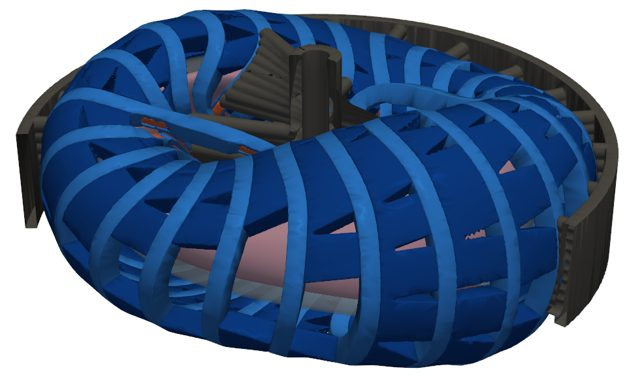
\includegraphics[width=\linewidth]{bilder/katalog/0009.jpg}\par\scriptsize \begin{tabular}{@{}l@{\,}r@{\quad}l@{\,}r@{}}Spulen & 24 & $\sigma_{99}$ & \num{1159} MPa \\Verb./Paar & 13 & max. & \num{9216} MPa \\$E_V$ & \num{145} GPa & Dehnung & \num{0.62} \% \\Abstand & \num{0.23} & $B\cdot n$ & \num{1.50} ‰ \\Stahl & \num{24} kt & frei & \num{1.55} m \\\end{tabular}\par verletzt: Stahl σ99, Dehnung Wickelpaket. PicoGK: keine Überschneidung.\end{minipage}\par\vspace{6pt}
\begin{minipage}[t]{0.47\linewidth}\textbf{0010} \hfill \num{-176}\,\%\par 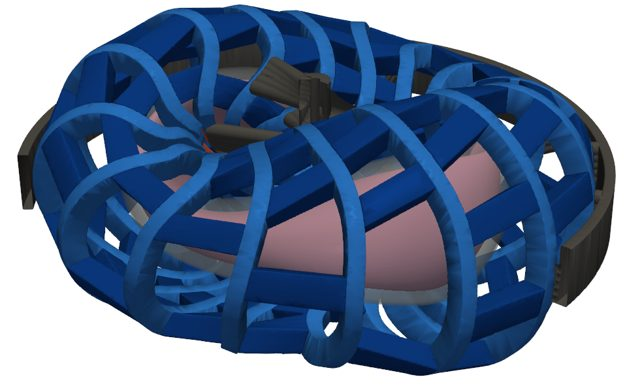
\includegraphics[width=\linewidth]{bilder/katalog/0010.jpg}\par\scriptsize \begin{tabular}{@{}l@{\,}r@{\quad}l@{\,}r@{}}Spulen & 16 & $\sigma_{99}$ & \num{1381} MPa \\Verb./Paar & 8 & max. & \num{8739} MPa \\$E_V$ & \num{149} GPa & Dehnung & \num{0.63} \% \\Abstand & \num{0.27} & $B\cdot n$ & \num{2.80} ‰ \\Stahl & \num{21} kt & frei & \num{1.93} m \\\end{tabular}\par verletzt: Stahl σ99, Dehnung Wickelpaket. PicoGK: keine Überschneidung.\end{minipage}\hfill
\begin{minipage}[t]{0.47\linewidth}\textbf{0011} \hfill \num{-519}\,\%\par 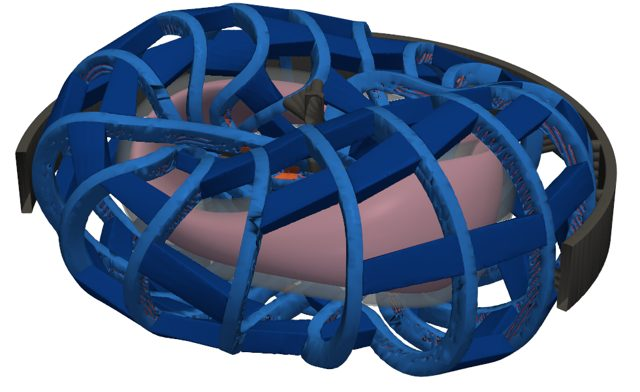
\includegraphics[width=\linewidth]{bilder/katalog/0011.jpg}\par\scriptsize \begin{tabular}{@{}l@{\,}r@{\quad}l@{\,}r@{}}Spulen & 16 & $\sigma_{99}$ & \num{3096} MPa \\Verb./Paar & 7 & max. & \num{19166} MPa \\$E_V$ & \num{42} GPa & Dehnung & \num{1.50} \% \\Abstand & \num{0.18} & $B\cdot n$ & \num{3.25} ‰ \\Stahl & \num{14} kt & frei & \num{1.80} m \\\end{tabular}\par verletzt: Stahl σ99, Dehnung Wickelpaket, Feldfehler B·n. PicoGK: keine Überschneidung.\end{minipage}\par\vspace{6pt}
\clearpage
\begin{minipage}[t]{0.47\linewidth}\textbf{0012} \hfill \num{-139}\,\%\par 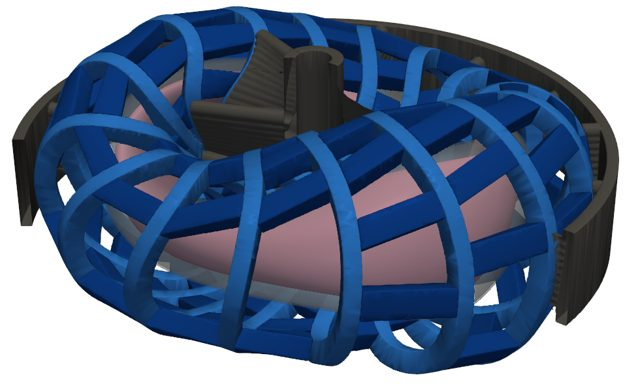
\includegraphics[width=\linewidth]{bilder/katalog/0012.jpg}\par\scriptsize \begin{tabular}{@{}l@{\,}r@{\quad}l@{\,}r@{}}Spulen & 16 & $\sigma_{99}$ & \num{999} MPa \\Verb./Paar & 9 & max. & \num{2952} MPa \\$E_V$ & \num{50} GPa & Dehnung & \num{0.40} \% \\Abstand & \num{0.21} & $B\cdot n$ & \num{7.17} ‰ \\Stahl & \num{13} kt & frei & \num{1.68} m \\\end{tabular}\par verletzt: Stahl σ99, Dehnung Wickelpaket, Feldfehler B·n. PicoGK: keine Überschneidung.\end{minipage}\hfill
\begin{minipage}[t]{0.47\linewidth}\textbf{0013} \hfill \num{-55}\,\%\par 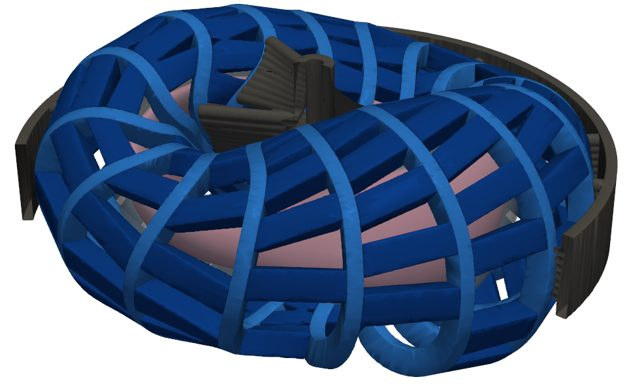
\includegraphics[width=\linewidth]{bilder/katalog/0013.jpg}\par\scriptsize \begin{tabular}{@{}l@{\,}r@{\quad}l@{\,}r@{}}Spulen & 16 & $\sigma_{99}$ & \num{773} MPa \\Verb./Paar & 14 & max. & \num{1718} MPa \\$E_V$ & \num{103} GPa & Dehnung & \num{0.34} \% \\Abstand & \num{0.13} & $B\cdot n$ & \num{4.32} ‰ \\Stahl & \num{25} kt & frei & \num{1.63} m \\\end{tabular}\par verletzt: Stahl σ99, Dehnung Wickelpaket, Feldfehler B·n. PicoGK: keine Überschneidung.\end{minipage}\par\vspace{6pt}
\begin{minipage}[t]{0.47\linewidth}\textbf{0014} \hfill \num{25}\,\%\par 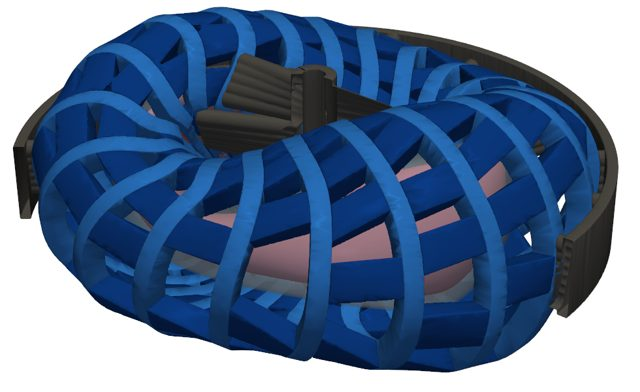
\includegraphics[width=\linewidth]{bilder/katalog/0014.jpg}\par\scriptsize \begin{tabular}{@{}l@{\,}r@{\quad}l@{\,}r@{}}Spulen & 20 & $\sigma_{99}$ & \num{377} MPa \\Verb./Paar & 11 & max. & \num{1419} MPa \\$E_V$ & \num{196} GPa & Dehnung & \num{0.21} \% \\Abstand & \num{0.23} & $B\cdot n$ & \num{2.21} ‰ \\Stahl & \num{28} kt & frei & \num{1.65} m \\\end{tabular}\par \textbf{zulässig}. PicoGK: keine Überschneidung.\end{minipage}\hfill
\begin{minipage}[t]{0.47\linewidth}\textbf{0015} \hfill \num{-628}\,\%\par 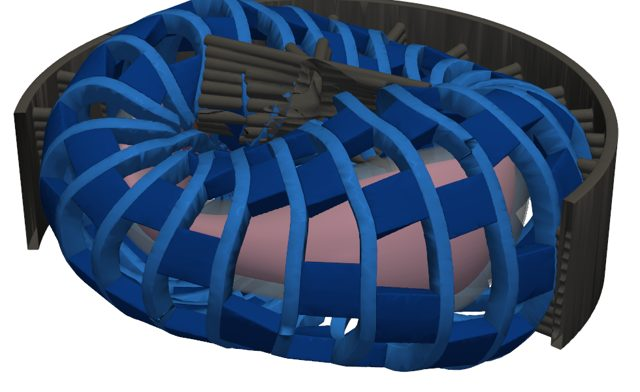
\includegraphics[width=\linewidth]{bilder/katalog/0015.jpg}\par\scriptsize \begin{tabular}{@{}l@{\,}r@{\quad}l@{\,}r@{}}Spulen & 24 & $\sigma_{99}$ & \num{3586} MPa \\Verb./Paar & 7 & max. & \num{30683} MPa \\$E_V$ & \num{168} GPa & Dehnung & \num{2.18} \% \\Abstand & \num{0.29} & $B\cdot n$ & \num{1.12} ‰ \\Stahl & \num{18} kt & frei & \num{2.48} m \\\end{tabular}\par verletzt: Stahl σ99, Dehnung Wickelpaket. PicoGK: keine Überschneidung.\end{minipage}\par\vspace{6pt}
\clearpage
\begin{minipage}[t]{0.47\linewidth}\textbf{0016} \hfill \num{-600}\,\%\par 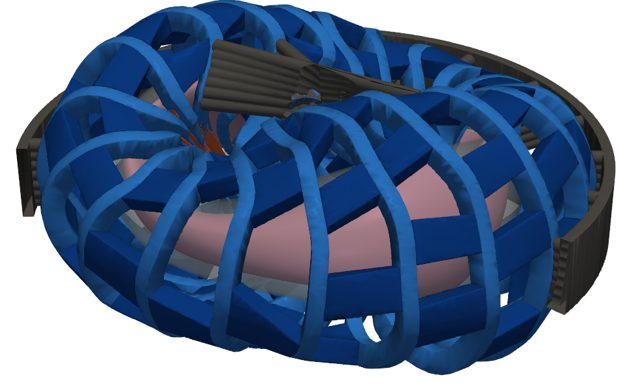
\includegraphics[width=\linewidth]{bilder/katalog/0016.jpg}\par\scriptsize \begin{tabular}{@{}l@{\,}r@{\quad}l@{\,}r@{}}Spulen & 20 & $\sigma_{99}$ & \num{3499} MPa \\Verb./Paar & 8 & max. & \num{15129} MPa \\$E_V$ & \num{172} GPa & Dehnung & \num{1.95} \% \\Abstand & \num{0.29} & $B\cdot n$ & \num{2.24} ‰ \\Stahl & \num{19} kt & frei & \num{2.42} m \\\end{tabular}\par verletzt: Stahl σ99, Dehnung Wickelpaket. PicoGK: keine Überschneidung.\end{minipage}\hfill
\begin{minipage}[t]{0.47\linewidth}\textbf{0017} \hfill \num{20}\,\%\par 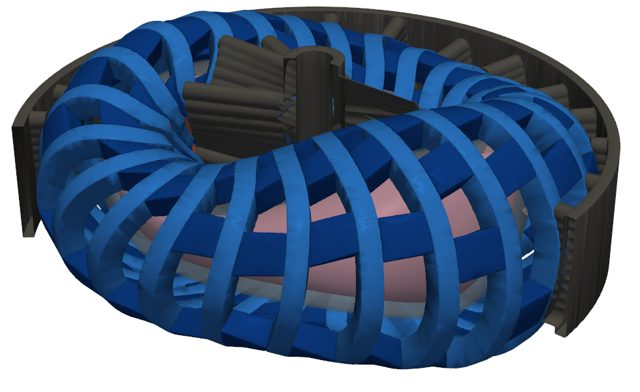
\includegraphics[width=\linewidth]{bilder/katalog/0017.jpg}\par\scriptsize \begin{tabular}{@{}l@{\,}r@{\quad}l@{\,}r@{}}Spulen & 24 & $\sigma_{99}$ & \num{389} MPa \\Verb./Paar & 7 & max. & \num{1721} MPa \\$E_V$ & \num{29} GPa & Dehnung & \num{0.20} \% \\Abstand & \num{0.22} & $B\cdot n$ & \num{1.66} ‰ \\Stahl & \num{23} kt & frei & \num{1.30} m \\\end{tabular}\par \textbf{zulässig}. PicoGK: keine Überschneidung.\end{minipage}\par\vspace{6pt}
\begin{minipage}[t]{0.47\linewidth}\textbf{0018}$^\ast$ \hfill \num{-99}\,\%\par 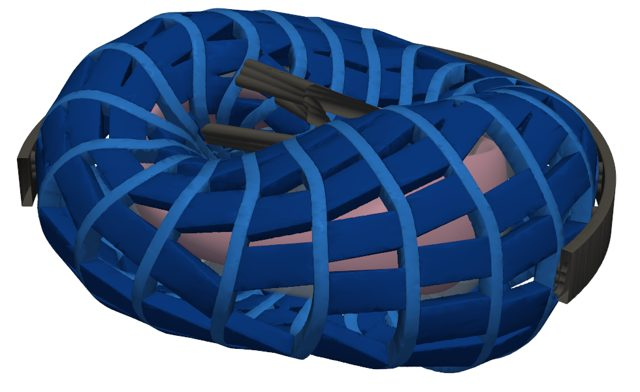
\includegraphics[width=\linewidth]{bilder/katalog/0018.jpg}\par\scriptsize \begin{tabular}{@{}l@{\,}r@{\quad}l@{\,}r@{}}Spulen & 20 & $\sigma_{99}$ & \num{996} MPa \\Verb./Paar & 14 & max. & \num{4566} MPa \\$E_V$ & \num{26} GPa & Dehnung & \num{0.44} \% \\Abstand & \num{0.25} & $B\cdot n$ & \num{1.43} ‰ \\Stahl & \num{24} kt & frei & \num{2.08} m \\\end{tabular}\par verletzt: Stahl σ99, Dehnung Wickelpaket. PicoGK: keine Überschneidung.\end{minipage}\hfill
\begin{minipage}[t]{0.47\linewidth}\textbf{0019} \hfill \num{-338}\,\%\par 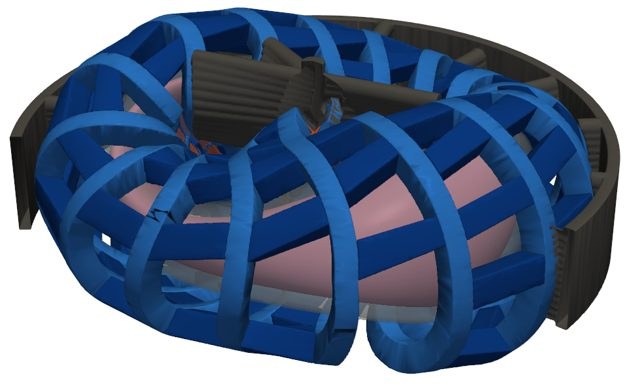
\includegraphics[width=\linewidth]{bilder/katalog/0019.jpg}\par\scriptsize \begin{tabular}{@{}l@{\,}r@{\quad}l@{\,}r@{}}Spulen & 16 & $\sigma_{99}$ & \num{1571} MPa \\Verb./Paar & 9 & max. & \num{14989} MPa \\$E_V$ & \num{24} GPa & Dehnung & \num{0.96} \% \\Abstand & \num{0.25} & $B\cdot n$ & \num{13.15} ‰ \\Stahl & \num{17} kt & frei & \num{1.93} m \\\end{tabular}\par verletzt: Stahl σ99, Dehnung Wickelpaket, Feldfehler B·n. PicoGK: keine Überschneidung.\end{minipage}\par\vspace{6pt}
\clearpage
\begin{minipage}[t]{0.47\linewidth}\textbf{0020} \hfill \num{-173}\,\%\par 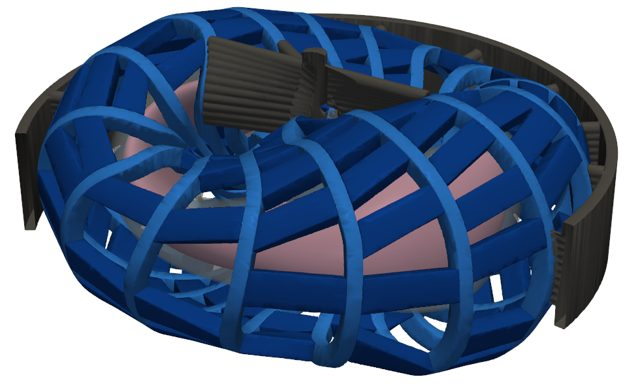
\includegraphics[width=\linewidth]{bilder/katalog/0020.jpg}\par\scriptsize \begin{tabular}{@{}l@{\,}r@{\quad}l@{\,}r@{}}Spulen & 16 & $\sigma_{99}$ & \num{1363} MPa \\Verb./Paar & 14 & max. & \num{6952} MPa \\$E_V$ & \num{137} GPa & Dehnung & \num{0.55} \% \\Abstand & \num{0.24} & $B\cdot n$ & \num{3.21} ‰ \\Stahl & \num{17} kt & frei & \num{1.78} m \\\end{tabular}\par verletzt: Stahl σ99, Dehnung Wickelpaket, Feldfehler B·n. PicoGK: keine Überschneidung.\end{minipage}\hfill
\begin{minipage}[t]{0.47\linewidth}\textbf{0021} \hfill \num{-4948}\,\%\par 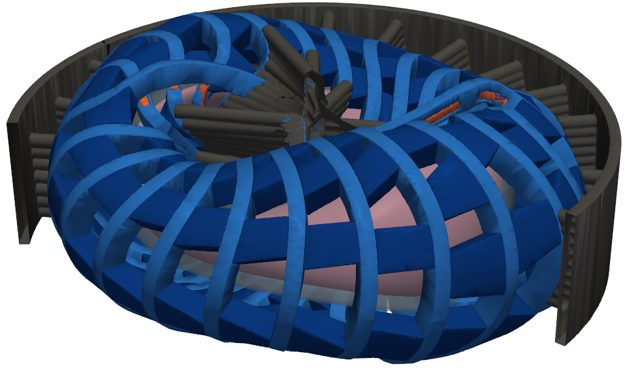
\includegraphics[width=\linewidth]{bilder/katalog/0021.jpg}\par\scriptsize \begin{tabular}{@{}l@{\,}r@{\quad}l@{\,}r@{}}Spulen & 24 & $\sigma_{99}$ & \num{558} MPa \\Verb./Paar & 8 & max. & \num{4173} MPa \\$E_V$ & \num{138} GPa & Dehnung & \num{0.29} \% \\Abstand & \num{0.16} & $B\cdot n$ & \num{2.26} ‰ \\Stahl & \num{26} kt & frei & \num{0.87} m \\\end{tabular}\par verletzt: Stahl σ99, Platz Package, Kernheizung, Neutronenfluenz. PicoGK: Überschneidung!\end{minipage}\par\vspace{6pt}
\begin{minipage}[t]{0.47\linewidth}\textbf{0022} \hfill \num{-20}\,\%\par 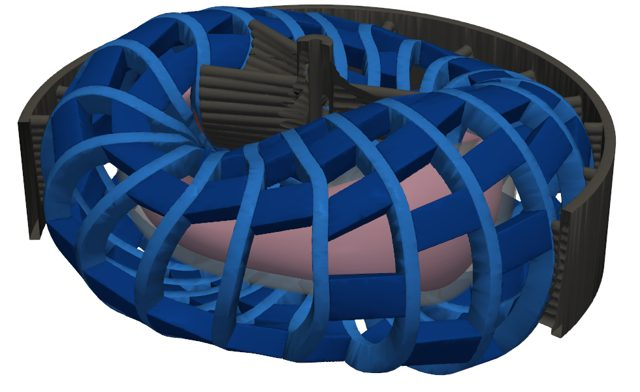
\includegraphics[width=\linewidth]{bilder/katalog/0022.jpg}\par\scriptsize \begin{tabular}{@{}l@{\,}r@{\quad}l@{\,}r@{}}Spulen & 20 & $\sigma_{99}$ & \num{600} MPa \\Verb./Paar & 8 & max. & \num{2183} MPa \\$E_V$ & \num{37} GPa & Dehnung & \num{0.26} \% \\Abstand & \num{0.23} & $B\cdot n$ & \num{0.70} ‰ \\Stahl & \num{24} kt & frei & \num{1.57} m \\\end{tabular}\par verletzt: Stahl σ99. PicoGK: keine Überschneidung.\end{minipage}\hfill
\begin{minipage}[t]{0.47\linewidth}\textbf{0023} \hfill \num{-276}\,\%\par 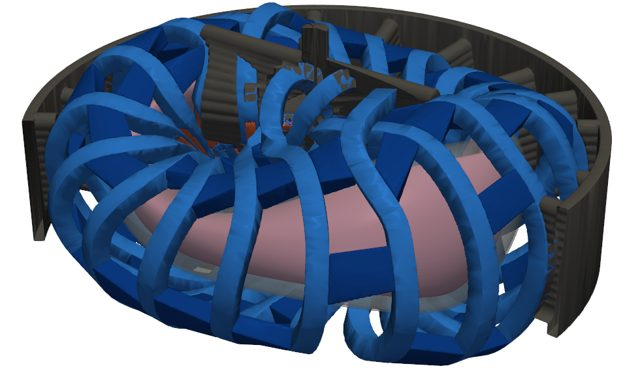
\includegraphics[width=\linewidth]{bilder/katalog/0023.jpg}\par\scriptsize \begin{tabular}{@{}l@{\,}r@{\quad}l@{\,}r@{}}Spulen & 20 & $\sigma_{99}$ & \num{1864} MPa \\Verb./Paar & 6 & max. & \num{10858} MPa \\$E_V$ & \num{156} GPa & Dehnung & \num{1.13} \% \\Abstand & \num{0.28} & $B\cdot n$ & \num{2.89} ‰ \\Stahl & \num{15} kt & frei & \num{2.06} m \\\end{tabular}\par verletzt: Stahl σ99, Dehnung Wickelpaket. PicoGK: keine Überschneidung.\end{minipage}\par\vspace{6pt}
\clearpage
\begin{minipage}[t]{0.47\linewidth}\textbf{0024} \hfill \num{-257}\,\%\par 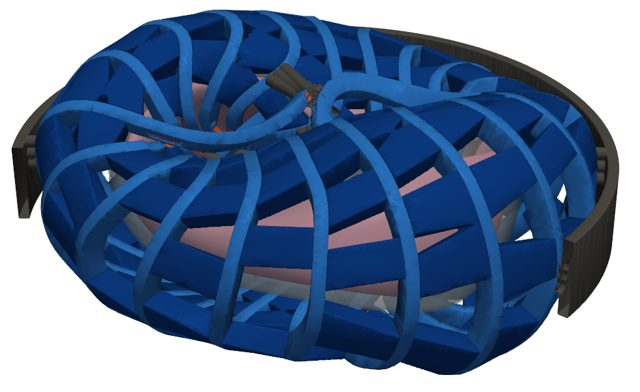
\includegraphics[width=\linewidth]{bilder/katalog/0024.jpg}\par\scriptsize \begin{tabular}{@{}l@{\,}r@{\quad}l@{\,}r@{}}Spulen & 20 & $\sigma_{99}$ & \num{1787} MPa \\Verb./Paar & 11 & max. & \num{7614} MPa \\$E_V$ & \num{24} GPa & Dehnung & \num{0.85} \% \\Abstand & \num{0.26} & $B\cdot n$ & \num{1.55} ‰ \\Stahl & \num{24} kt & frei & \num{1.82} m \\\end{tabular}\par verletzt: Stahl σ99, Dehnung Wickelpaket. PicoGK: keine Überschneidung.\end{minipage}\hfill
\begin{minipage}[t]{0.47\linewidth}\textbf{0025} \hfill \num{-102}\,\%\par 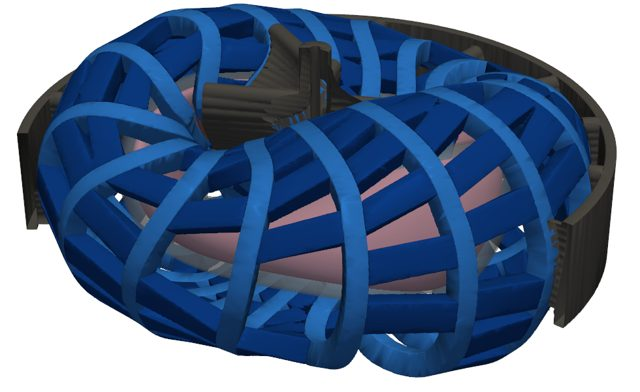
\includegraphics[width=\linewidth]{bilder/katalog/0025.jpg}\par\scriptsize \begin{tabular}{@{}l@{\,}r@{\quad}l@{\,}r@{}}Spulen & 16 & $\sigma_{99}$ & \num{1010} MPa \\Verb./Paar & 14 & max. & \num{9842} MPa \\$E_V$ & \num{41} GPa & Dehnung & \num{0.50} \% \\Abstand & \num{0.18} & $B\cdot n$ & \num{1.94} ‰ \\Stahl & \num{26} kt & frei & \num{1.88} m \\\end{tabular}\par verletzt: Stahl σ99, Dehnung Wickelpaket. PicoGK: keine Überschneidung.\end{minipage}\par\vspace{6pt}
\begin{minipage}[t]{0.47\linewidth}\textbf{0026} \hfill \num{-62}\,\%\par 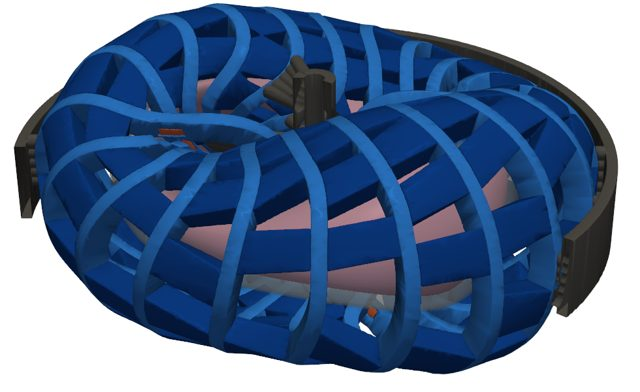
\includegraphics[width=\linewidth]{bilder/katalog/0026.jpg}\par\scriptsize \begin{tabular}{@{}l@{\,}r@{\quad}l@{\,}r@{}}Spulen & 20 & $\sigma_{99}$ & \num{809} MPa \\Verb./Paar & 11 & max. & \num{2253} MPa \\$E_V$ & \num{79} GPa & Dehnung & \num{0.38} \% \\Abstand & \num{0.19} & $B\cdot n$ & \num{1.43} ‰ \\Stahl & \num{29} kt & frei & \num{1.41} m \\\end{tabular}\par verletzt: Stahl σ99, Dehnung Wickelpaket. PicoGK: keine Überschneidung.\end{minipage}\hfill
\begin{minipage}[t]{0.47\linewidth}\textbf{0027} \hfill \num{-316}\,\%\par 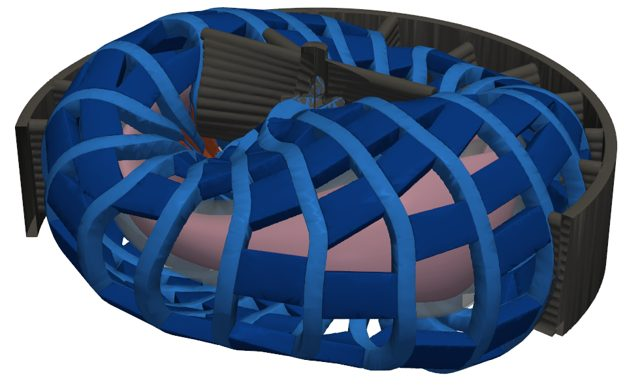
\includegraphics[width=\linewidth]{bilder/katalog/0027.jpg}\par\scriptsize \begin{tabular}{@{}l@{\,}r@{\quad}l@{\,}r@{}}Spulen & 20 & $\sigma_{99}$ & \num{2080} MPa \\Verb./Paar & 10 & max. & \num{10143} MPa \\$E_V$ & \num{171} GPa & Dehnung & \num{1.02} \% \\Abstand & \num{0.28} & $B\cdot n$ & \num{2.25} ‰ \\Stahl & \num{16} kt & frei & \num{2.18} m \\\end{tabular}\par verletzt: Stahl σ99, Dehnung Wickelpaket. PicoGK: keine Überschneidung.\end{minipage}\par\vspace{6pt}
\clearpage
\begin{minipage}[t]{0.47\linewidth}\textbf{0028} \hfill \num{-78}\,\%\par 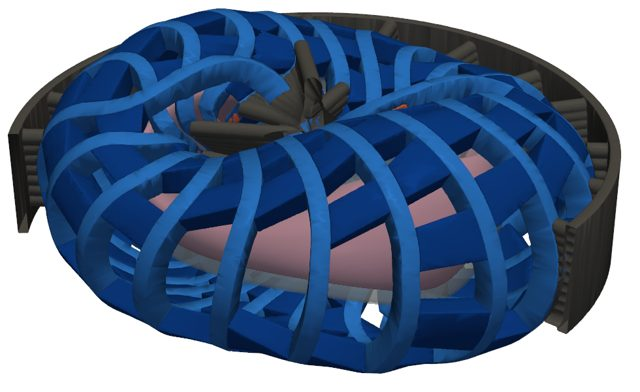
\includegraphics[width=\linewidth]{bilder/katalog/0028.jpg}\par\scriptsize \begin{tabular}{@{}l@{\,}r@{\quad}l@{\,}r@{}}Spulen & 20 & $\sigma_{99}$ & \num{888} MPa \\Verb./Paar & 9 & max. & \num{3682} MPa \\$E_V$ & \num{22} GPa & Dehnung & \num{0.40} \% \\Abstand & \num{0.17} & $B\cdot n$ & \num{1.45} ‰ \\Stahl & \num{30} kt & frei & \num{1.33} m \\\end{tabular}\par verletzt: Stahl σ99, Dehnung Wickelpaket. PicoGK: keine Überschneidung.\end{minipage}\hfill
\begin{minipage}[t]{0.47\linewidth}\textbf{0029} \hfill \num{-361}\,\%\par 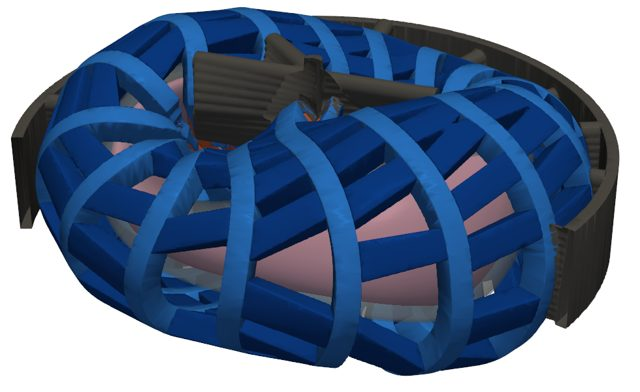
\includegraphics[width=\linewidth]{bilder/katalog/0029.jpg}\par\scriptsize \begin{tabular}{@{}l@{\,}r@{\quad}l@{\,}r@{}}Spulen & 16 & $\sigma_{99}$ & \num{1975} MPa \\Verb./Paar & 13 & max. & \num{34584} MPa \\$E_V$ & \num{27} GPa & Dehnung & \num{1.38} \% \\Abstand & \num{0.29} & $B\cdot n$ & \num{10.34} ‰ \\Stahl & \num{22} kt & frei & \num{2.35} m \\\end{tabular}\par verletzt: Stahl σ99, Dehnung Wickelpaket, Feldfehler B·n. PicoGK: keine Überschneidung.\end{minipage}\par\vspace{6pt}
\begin{minipage}[t]{0.47\linewidth}\textbf{0031} \hfill \num{-222}\,\%\par 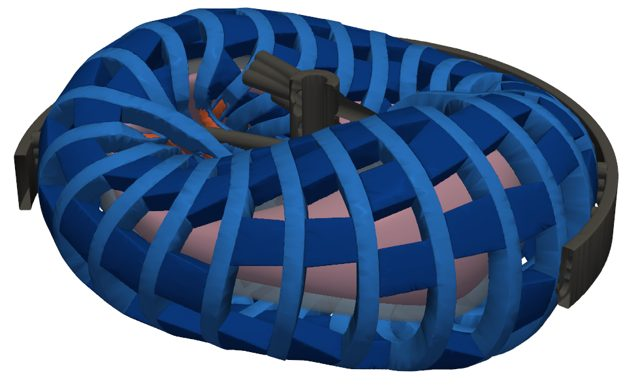
\includegraphics[width=\linewidth]{bilder/katalog/0031.jpg}\par\scriptsize \begin{tabular}{@{}l@{\,}r@{\quad}l@{\,}r@{}}Spulen & 24 & $\sigma_{99}$ & \num{1514} MPa \\Verb./Paar & 8 & max. & \num{8426} MPa \\$E_V$ & \num{190} GPa & Dehnung & \num{0.97} \% \\Abstand & \num{0.24} & $B\cdot n$ & \num{1.99} ‰ \\Stahl & \num{21} kt & frei & \num{1.84} m \\\end{tabular}\par verletzt: Stahl σ99, Dehnung Wickelpaket. PicoGK: keine Überschneidung.\end{minipage}\hfill
\begin{minipage}[t]{0.47\linewidth}\textbf{0032} \hfill \num{-123}\,\%\par 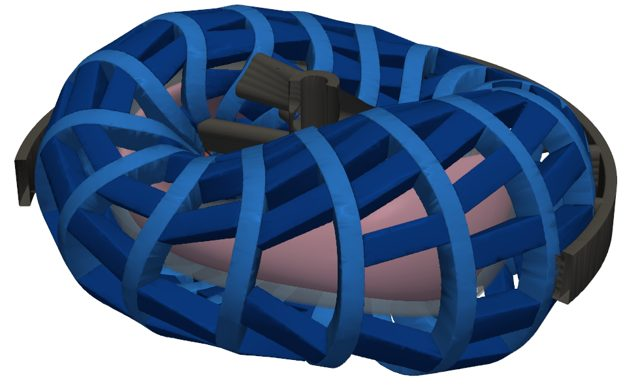
\includegraphics[width=\linewidth]{bilder/katalog/0032.jpg}\par\scriptsize \begin{tabular}{@{}l@{\,}r@{\quad}l@{\,}r@{}}Spulen & 16 & $\sigma_{99}$ & \num{777} MPa \\Verb./Paar & 12 & max. & \num{3008} MPa \\$E_V$ & \num{38} GPa & Dehnung & \num{0.28} \% \\Abstand & \num{0.17} & $B\cdot n$ & \num{6.70} ‰ \\Stahl & \num{25} kt & frei & \num{1.48} m \\\end{tabular}\par verletzt: Stahl σ99, Feldfehler B·n. PicoGK: keine Überschneidung.\end{minipage}\par\vspace{6pt}
\clearpage
\begin{minipage}[t]{0.47\linewidth}\textbf{0033} \hfill \num{-125}\,\%\par 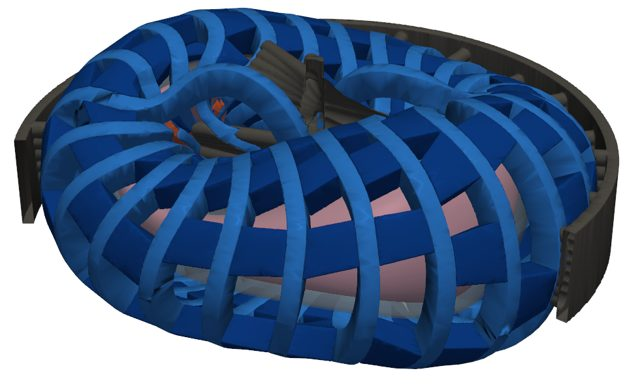
\includegraphics[width=\linewidth]{bilder/katalog/0033.jpg}\par\scriptsize \begin{tabular}{@{}l@{\,}r@{\quad}l@{\,}r@{}}Spulen & 24 & $\sigma_{99}$ & \num{1019} MPa \\Verb./Paar & 8 & max. & \num{4409} MPa \\$E_V$ & \num{118} GPa & Dehnung & \num{0.68} \% \\Abstand & \num{0.25} & $B\cdot n$ & \num{1.78} ‰ \\Stahl & \num{25} kt & frei & \num{1.56} m \\\end{tabular}\par verletzt: Stahl σ99, Dehnung Wickelpaket. PicoGK: keine Überschneidung.\end{minipage}\hfill
\begin{minipage}[t]{0.47\linewidth}\textbf{0034} \hfill \num{-215}\,\%\par \par\scriptsize \begin{tabular}{@{}l@{\,}r@{\quad}l@{\,}r@{}}Spulen & 16 & $\sigma_{99}$ & \num{1574} MPa \\Verb./Paar & 6 & max. & \num{4775} MPa \\$E_V$ & \num{21} GPa & Dehnung & \num{0.56} \% \\Abstand & \num{0.26} & $B\cdot n$ & \num{3.08} ‰ \\Stahl & \num{17} kt & frei & \num{1.96} m \\\end{tabular}\par verletzt: Stahl σ99, Dehnung Wickelpaket, Feldfehler B·n.\end{minipage}\par\vspace{6pt}
\begin{minipage}[t]{0.47\linewidth}\textbf{0035} \hfill \num{-278}\,\%\par \par\scriptsize \begin{tabular}{@{}l@{\,}r@{\quad}l@{\,}r@{}}Spulen & 24 & $\sigma_{99}$ & \num{1892} MPa \\Verb./Paar & 12 & max. & \num{5956} MPa \\$E_V$ & \num{50} GPa & Dehnung & \num{0.83} \% \\Abstand & \num{0.18} & $B\cdot n$ & \num{1.23} ‰ \\Stahl & \num{30} kt & frei & \num{1.31} m \\\end{tabular}\par verletzt: Stahl σ99, Dehnung Wickelpaket.\end{minipage}\hfill
\begin{minipage}[t]{0.47\linewidth}\textbf{0036} \hfill \num{-37}\,\%\par \par\scriptsize \begin{tabular}{@{}l@{\,}r@{\quad}l@{\,}r@{}}Spulen & 20 & $\sigma_{99}$ & \num{683} MPa \\Verb./Paar & 7 & max. & \num{7457} MPa \\$E_V$ & \num{119} GPa & Dehnung & \num{0.38} \% \\Abstand & \num{0.25} & $B\cdot n$ & \num{3.45} ‰ \\Stahl & \num{15} kt & frei & \num{1.74} m \\\end{tabular}\par verletzt: Stahl σ99, Dehnung Wickelpaket, Feldfehler B·n.\end{minipage}\par\vspace{6pt}
\clearpage
\begin{minipage}[t]{0.47\linewidth}\textbf{0037} \hfill \num{-260}\,\%\par \par\scriptsize \begin{tabular}{@{}l@{\,}r@{\quad}l@{\,}r@{}}Spulen & 24 & $\sigma_{99}$ & \num{1800} MPa \\Verb./Paar & 6 & max. & \num{4950} MPa \\$E_V$ & \num{53} GPa & Dehnung & \num{0.66} \% \\Abstand & \num{0.13} & $B\cdot n$ & \num{1.33} ‰ \\Stahl & \num{12} kt & frei & \num{1.43} m \\\end{tabular}\par verletzt: Stahl σ99, Dehnung Wickelpaket.\end{minipage}\hfill
\begin{minipage}[t]{0.47\linewidth}\textbf{0038} \hfill \num{-204}\,\%\par \par\scriptsize \begin{tabular}{@{}l@{\,}r@{\quad}l@{\,}r@{}}Spulen & 20 & $\sigma_{99}$ & \num{525} MPa \\Verb./Paar & 13 & max. & \num{2561} MPa \\$E_V$ & \num{60} GPa & Dehnung & \num{0.23} \% \\Abstand & \num{0.17} & $B\cdot n$ & \num{3.27} ‰ \\Stahl & \num{32} kt & frei & \num{1.15} m \\\end{tabular}\par verletzt: Stahl σ99, Neutronenfluenz, Feldfehler B·n.\end{minipage}\par\vspace{6pt}
\begin{minipage}[t]{0.47\linewidth}\textbf{0039} \hfill \num{-210}\,\%\par \par\scriptsize \begin{tabular}{@{}l@{\,}r@{\quad}l@{\,}r@{}}Spulen & 16 & $\sigma_{99}$ & \num{1548} MPa \\Verb./Paar & 7 & max. & \num{6664} MPa \\$E_V$ & \num{31} GPa & Dehnung & \num{0.70} \% \\Abstand & \num{0.28} & $B\cdot n$ & \num{4.38} ‰ \\Stahl & \num{14} kt & frei & \num{2.05} m \\\end{tabular}\par verletzt: Stahl σ99, Dehnung Wickelpaket, Feldfehler B·n.\end{minipage}\hfill
\begin{minipage}[t]{0.47\linewidth}\textbf{0040} \hfill \num{-240}\,\%\par \par\scriptsize \begin{tabular}{@{}l@{\,}r@{\quad}l@{\,}r@{}}Spulen & 24 & $\sigma_{99}$ & \num{1262} MPa \\Verb./Paar & 12 & max. & \num{9182} MPa \\$E_V$ & \num{91} GPa & Dehnung & \num{1.02} \% \\Abstand & \num{0.29} & $B\cdot n$ & \num{3.84} ‰ \\Stahl & \num{23} kt & frei & \num{2.41} m \\\end{tabular}\par verletzt: Stahl σ99, Dehnung Wickelpaket, Feldfehler B·n.\end{minipage}\par\vspace{6pt}
\clearpage
\begin{minipage}[t]{0.47\linewidth}\textbf{0041} \hfill \num{-69}\,\%\par \par\scriptsize \begin{tabular}{@{}l@{\,}r@{\quad}l@{\,}r@{}}Spulen & 16 & $\sigma_{99}$ & \num{843} MPa \\Verb./Paar & 9 & max. & \num{1629} MPa \\$E_V$ & \num{73} GPa & Dehnung & \num{0.36} \% \\Abstand & \num{0.14} & $B\cdot n$ & \num{4.96} ‰ \\Stahl & \num{13} kt & frei & \num{1.60} m \\\end{tabular}\par verletzt: Stahl σ99, Dehnung Wickelpaket, Feldfehler B·n.\end{minipage}\hfill
\begin{minipage}[t]{0.47\linewidth}\textbf{0042} \hfill \num{-26}\,\%\par \par\scriptsize \begin{tabular}{@{}l@{\,}r@{\quad}l@{\,}r@{}}Spulen & 20 & $\sigma_{99}$ & \num{632} MPa \\Verb./Paar & 12 & max. & \num{3962} MPa \\$E_V$ & \num{170} GPa & Dehnung & \num{0.34} \% \\Abstand & \num{0.14} & $B\cdot n$ & \num{2.66} ‰ \\Stahl & \num{21} kt & frei & \num{1.61} m \\\end{tabular}\par verletzt: Stahl σ99, Dehnung Wickelpaket.\end{minipage}\par\vspace{6pt}
\begin{minipage}[t]{0.47\linewidth}\textbf{0043} \hfill \num{-31}\,\%\par \par\scriptsize \begin{tabular}{@{}l@{\,}r@{\quad}l@{\,}r@{}}Spulen & 24 & $\sigma_{99}$ & \num{653} MPa \\Verb./Paar & 9 & max. & \num{1208} MPa \\$E_V$ & \num{40} GPa & Dehnung & \num{0.29} \% \\Abstand & \num{0.17} & $B\cdot n$ & \num{1.79} ‰ \\Stahl & \num{16} kt & frei & \num{1.30} m \\\end{tabular}\par verletzt: Stahl σ99.\end{minipage}\hfill
\begin{minipage}[t]{0.47\linewidth}\textbf{0044} \hfill \num{-8}\,\%\par \par\scriptsize \begin{tabular}{@{}l@{\,}r@{\quad}l@{\,}r@{}}Spulen & 20 & $\sigma_{99}$ & \num{540} MPa \\Verb./Paar & 13 & max. & \num{1583} MPa \\$E_V$ & \num{110} GPa & Dehnung & \num{0.23} \% \\Abstand & \num{0.16} & $B\cdot n$ & \num{2.76} ‰ \\Stahl & \num{26} kt & frei & \num{1.35} m \\\end{tabular}\par verletzt: Stahl σ99.\end{minipage}\par\vspace{6pt}
\clearpage
\begin{minipage}[t]{0.47\linewidth}\textbf{0045} \hfill \num{-58}\,\%\par \par\scriptsize \begin{tabular}{@{}l@{\,}r@{\quad}l@{\,}r@{}}Spulen & 20 & $\sigma_{99}$ & \num{600} MPa \\Verb./Paar & 9 & max. & \num{3060} MPa \\$E_V$ & \num{175} GPa & Dehnung & \num{0.29} \% \\Abstand & \num{0.15} & $B\cdot n$ & \num{4.74} ‰ \\Stahl & \num{22} kt & frei & \num{1.36} m \\\end{tabular}\par verletzt: Stahl σ99, Feldfehler B·n.\end{minipage}\hfill
\begin{minipage}[t]{0.47\linewidth}\textbf{0046} \hfill \num{-112}\,\%\par \par\scriptsize \begin{tabular}{@{}l@{\,}r@{\quad}l@{\,}r@{}}Spulen & 16 & $\sigma_{99}$ & \num{619} MPa \\Verb./Paar & 9 & max. & \num{2502} MPa \\$E_V$ & \num{46} GPa & Dehnung & \num{0.26} \% \\Abstand & \num{0.16} & $B\cdot n$ & \num{6.36} ‰ \\Stahl & \num{22} kt & frei & \num{1.43} m \\\end{tabular}\par verletzt: Stahl σ99, Feldfehler B·n.\end{minipage}\par\vspace{6pt}
\begin{minipage}[t]{0.47\linewidth}\textbf{0047} \hfill \num{-407}\,\%\par \par\scriptsize \begin{tabular}{@{}l@{\,}r@{\quad}l@{\,}r@{}}Spulen & 24 & $\sigma_{99}$ & \num{983} MPa \\Verb./Paar & 8 & max. & \num{4736} MPa \\$E_V$ & \num{34} GPa & Dehnung & \num{0.42} \% \\Abstand & \num{0.15} & $B\cdot n$ & \num{1.48} ‰ \\Stahl & \num{25} kt & frei & \num{1.10} m \\\end{tabular}\par verletzt: Stahl σ99, Dehnung Wickelpaket, Platz Package, Neutronenfluenz.\end{minipage}\hfill
\begin{minipage}[t]{0.47\linewidth}\textbf{0048} \hfill \num{-364}\,\%\par \par\scriptsize \begin{tabular}{@{}l@{\,}r@{\quad}l@{\,}r@{}}Spulen & 16 & $\sigma_{99}$ & \num{2081} MPa \\Verb./Paar & 7 & max. & \num{19844} MPa \\$E_V$ & \num{160} GPa & Dehnung & \num{1.39} \% \\Abstand & \num{0.29} & $B\cdot n$ & \num{10.18} ‰ \\Stahl & \num{13} kt & frei & \num{2.32} m \\\end{tabular}\par verletzt: Stahl σ99, Dehnung Wickelpaket, Feldfehler B·n.\end{minipage}\par\vspace{6pt}
\clearpage
\begin{minipage}[t]{0.47\linewidth}\textbf{0049} \hfill \num{-462}\,\%\par \par\scriptsize \begin{tabular}{@{}l@{\,}r@{\quad}l@{\,}r@{}}Spulen & 16 & $\sigma_{99}$ & \num{2808} MPa \\Verb./Paar & 9 & max. & \num{9212} MPa \\$E_V$ & \num{84} GPa & Dehnung & \num{1.07} \% \\Abstand & \num{0.21} & $B\cdot n$ & \num{2.42} ‰ \\Stahl & \num{18} kt & frei & \num{1.74} m \\\end{tabular}\par verletzt: Stahl σ99, Dehnung Wickelpaket.\end{minipage}\hfill
\begin{minipage}[t]{0.47\linewidth}\textbf{0051} \hfill \num{-130}\,\%\par \par\scriptsize \begin{tabular}{@{}l@{\,}r@{\quad}l@{\,}r@{}}Spulen & 20 & $\sigma_{99}$ & \num{1152} MPa \\Verb./Paar & 10 & max. & \num{2169} MPa \\$E_V$ & \num{37} GPa & Dehnung & \num{0.50} \% \\Abstand & \num{0.17} & $B\cdot n$ & \num{3.32} ‰ \\Stahl & \num{15} kt & frei & \num{1.50} m \\\end{tabular}\par verletzt: Stahl σ99, Dehnung Wickelpaket, Feldfehler B·n.\end{minipage}\par\vspace{6pt}
\begin{minipage}[t]{0.47\linewidth}\textbf{0052} \hfill \num{-164}\,\%\par \par\scriptsize \begin{tabular}{@{}l@{\,}r@{\quad}l@{\,}r@{}}Spulen & 24 & $\sigma_{99}$ & \num{1321} MPa \\Verb./Paar & 13 & max. & \num{4323} MPa \\$E_V$ & \num{55} GPa & Dehnung & \num{0.52} \% \\Abstand & \num{0.19} & $B\cdot n$ & \num{2.06} ‰ \\Stahl & \num{20} kt & frei & \num{1.39} m \\\end{tabular}\par verletzt: Stahl σ99, Dehnung Wickelpaket.\end{minipage}\hfill
\begin{minipage}[t]{0.47\linewidth}\textbf{0053} \hfill \num{-163}\,\%\par \par\scriptsize \begin{tabular}{@{}l@{\,}r@{\quad}l@{\,}r@{}}Spulen & 20 & $\sigma_{99}$ & \num{1314} MPa \\Verb./Paar & 6 & max. & \num{9639} MPa \\$E_V$ & \num{57} GPa & Dehnung & \num{0.57} \% \\Abstand & \num{0.25} & $B\cdot n$ & \num{1.71} ‰ \\Stahl & \num{11} kt & frei & \num{2.02} m \\\end{tabular}\par verletzt: Stahl σ99, Dehnung Wickelpaket.\end{minipage}\par\vspace{6pt}
\clearpage
\begin{minipage}[t]{0.47\linewidth}\textbf{0054} \hfill \num{-138}\,\%\par \par\scriptsize \begin{tabular}{@{}l@{\,}r@{\quad}l@{\,}r@{}}Spulen & 16 & $\sigma_{99}$ & \num{963} MPa \\Verb./Paar & 7 & max. & \num{2479} MPa \\$E_V$ & \num{62} GPa & Dehnung & \num{0.37} \% \\Abstand & \num{0.16} & $B\cdot n$ & \num{7.15} ‰ \\Stahl & \num{12} kt & frei & \num{1.42} m \\\end{tabular}\par verletzt: Stahl σ99, Dehnung Wickelpaket, Feldfehler B·n.\end{minipage}\hfill
\begin{minipage}[t]{0.47\linewidth}\textbf{0055}$^\ast$ \hfill \num{-192}\,\%\par \par\scriptsize \begin{tabular}{@{}l@{\,}r@{\quad}l@{\,}r@{}}Spulen & 20 & $\sigma_{99}$ & \num{413} MPa \\Verb./Paar & 14 & max. & \num{942} MPa \\$E_V$ & \num{38} GPa & Dehnung & \num{0.18} \% \\Abstand & \num{0.13} & $B\cdot n$ & \num{2.84} ‰ \\Stahl & \num{32} kt & frei & \num{1.15} m \\\end{tabular}\par verletzt: Neutronenfluenz.\end{minipage}\par\vspace{6pt}
\begin{minipage}[t]{0.47\linewidth}\textbf{0056} \hfill \num{-423}\,\%\par \par\scriptsize \begin{tabular}{@{}l@{\,}r@{\quad}l@{\,}r@{}}Spulen & 20 & $\sigma_{99}$ & \num{2615} MPa \\Verb./Paar & 8 & max. & \num{13038} MPa \\$E_V$ & \num{59} GPa & Dehnung & \num{1.21} \% \\Abstand & \num{0.28} & $B\cdot n$ & \num{2.25} ‰ \\Stahl & \num{16} kt & frei & \num{2.06} m \\\end{tabular}\par verletzt: Stahl σ99, Dehnung Wickelpaket.\end{minipage}\hfill
\begin{minipage}[t]{0.47\linewidth}\textbf{0057} \hfill \num{-111}\,\%\par \par\scriptsize \begin{tabular}{@{}l@{\,}r@{\quad}l@{\,}r@{}}Spulen & 20 & $\sigma_{99}$ & \num{1056} MPa \\Verb./Paar & 6 & max. & \num{4063} MPa \\$E_V$ & \num{31} GPa & Dehnung & \num{0.39} \% \\Abstand & \num{0.24} & $B\cdot n$ & \num{2.18} ‰ \\Stahl & \num{14} kt & frei & \num{1.60} m \\\end{tabular}\par verletzt: Stahl σ99, Dehnung Wickelpaket.\end{minipage}\par\vspace{6pt}
\clearpage
\begin{minipage}[t]{0.47\linewidth}\textbf{0058} \hfill \num{-124}\,\%\par \par\scriptsize \begin{tabular}{@{}l@{\,}r@{\quad}l@{\,}r@{}}Spulen & 16 & $\sigma_{99}$ & \num{689} MPa \\Verb./Paar & 10 & max. & \num{2099} MPa \\$E_V$ & \num{32} GPa & Dehnung & \num{0.29} \% \\Abstand & \num{0.23} & $B\cdot n$ & \num{6.71} ‰ \\Stahl & \num{29} kt & frei & \num{1.60} m \\\end{tabular}\par verletzt: Stahl σ99, Feldfehler B·n.\end{minipage}\hfill
\begin{minipage}[t]{0.47\linewidth}\textbf{0059} \hfill \num{-132}\,\%\par \par\scriptsize \begin{tabular}{@{}l@{\,}r@{\quad}l@{\,}r@{}}Spulen & 16 & $\sigma_{99}$ & \num{1161} MPa \\Verb./Paar & 11 & max. & \num{4304} MPa \\$E_V$ & \num{110} GPa & Dehnung & \num{0.57} \% \\Abstand & \num{0.19} & $B\cdot n$ & \num{2.27} ‰ \\Stahl & \num{31} kt & frei & \num{1.48} m \\\end{tabular}\par verletzt: Stahl σ99, Dehnung Wickelpaket.\end{minipage}\par\vspace{6pt}
\begin{minipage}[t]{0.47\linewidth}\textbf{0060}$^\ast$ \hfill \num{-41}\,\%\par \par\scriptsize \begin{tabular}{@{}l@{\,}r@{\quad}l@{\,}r@{}}Spulen & 24 & $\sigma_{99}$ & \num{704} MPa \\Verb./Paar & 13 & max. & \num{1499} MPa \\$E_V$ & \num{155} GPa & Dehnung & \num{0.29} \% \\Abstand & \num{0.22} & $B\cdot n$ & \num{1.61} ‰ \\Stahl & \num{16} kt & frei & \num{1.66} m \\\end{tabular}\par verletzt: Stahl σ99.\end{minipage}\hfill
\begin{minipage}[t]{0.47\linewidth}\textbf{0061} \hfill \num{30}\,\%\par \par\scriptsize \begin{tabular}{@{}l@{\,}r@{\quad}l@{\,}r@{}}Spulen & 24 & $\sigma_{99}$ & \num{351} MPa \\Verb./Paar & 10 & max. & \num{725} MPa \\$E_V$ & \num{93} GPa & Dehnung & \num{0.17} \% \\Abstand & \num{0.20} & $B\cdot n$ & \num{1.49} ‰ \\Stahl & \num{19} kt & frei & \num{1.62} m \\\end{tabular}\par \textbf{zulässig}.\end{minipage}\par\vspace{6pt}
\clearpage
\begin{minipage}[t]{0.47\linewidth}\textbf{0062} \hfill \num{-427}\,\%\par \par\scriptsize \begin{tabular}{@{}l@{\,}r@{\quad}l@{\,}r@{}}Spulen & 24 & $\sigma_{99}$ & \num{2627} MPa \\Verb./Paar & 9 & max. & \num{13807} MPa \\$E_V$ & \num{21} GPa & Dehnung & \num{1.58} \% \\Abstand & \num{0.30} & $B\cdot n$ & \num{3.27} ‰ \\Stahl & \num{17} kt & frei & \num{2.40} m \\\end{tabular}\par verletzt: Stahl σ99, Dehnung Wickelpaket, Feldfehler B·n.\end{minipage}\hfill
\begin{minipage}[t]{0.47\linewidth}\textbf{0063}$^\ast$ \hfill \num{-24}\,\%\par \par\scriptsize \begin{tabular}{@{}l@{\,}r@{\quad}l@{\,}r@{}}Spulen & 20 & $\sigma_{99}$ & \num{595} MPa \\Verb./Paar & 14 & max. & \num{4265} MPa \\$E_V$ & \num{43} GPa & Dehnung & \num{0.37} \% \\Abstand & \num{0.18} & $B\cdot n$ & \num{0.75} ‰ \\Stahl & \num{41} kt & frei & \num{1.53} m \\\end{tabular}\par verletzt: Stahl σ99, Dehnung Wickelpaket.\end{minipage}\par\vspace{6pt}
\begin{minipage}[t]{0.47\linewidth}\textbf{0064} \hfill \num{-90}\,\%\par \par\scriptsize \begin{tabular}{@{}l@{\,}r@{\quad}l@{\,}r@{}}Spulen & 16 & $\sigma_{99}$ & \num{683} MPa \\Verb./Paar & 12 & max. & \num{5601} MPa \\$E_V$ & \num{131} GPa & Dehnung & \num{0.35} \% \\Abstand & \num{0.27} & $B\cdot n$ & \num{5.70} ‰ \\Stahl & \num{22} kt & frei & \num{1.85} m \\\end{tabular}\par verletzt: Stahl σ99, Dehnung Wickelpaket, Feldfehler B·n.\end{minipage}\hfill
\begin{minipage}[t]{0.47\linewidth}\textbf{0065} \hfill \num{-32}\,\%\par \par\scriptsize \begin{tabular}{@{}l@{\,}r@{\quad}l@{\,}r@{}}Spulen & 20 & $\sigma_{99}$ & \num{660} MPa \\Verb./Paar & 9 & max. & \num{1210} MPa \\$E_V$ & \num{48} GPa & Dehnung & \num{0.31} \% \\Abstand & \num{0.17} & $B\cdot n$ & \num{1.97} ‰ \\Stahl & \num{15} kt & frei & \num{1.61} m \\\end{tabular}\par verletzt: Stahl σ99, Dehnung Wickelpaket.\end{minipage}\par\vspace{6pt}
\clearpage
\begin{minipage}[t]{0.47\linewidth}\textbf{0067} \hfill \num{-100}\,\%\par \par\scriptsize \begin{tabular}{@{}l@{\,}r@{\quad}l@{\,}r@{}}Spulen & 20 & $\sigma_{99}$ & \num{999} MPa \\Verb./Paar & 11 & max. & \num{2826} MPa \\$E_V$ & \num{82} GPa & Dehnung & \num{0.47} \% \\Abstand & \num{0.20} & $B\cdot n$ & \num{3.08} ‰ \\Stahl & \num{28} kt & frei & \num{1.53} m \\\end{tabular}\par verletzt: Stahl σ99, Dehnung Wickelpaket, Feldfehler B·n.\end{minipage}\hfill
\begin{minipage}[t]{0.47\linewidth}\textbf{0068} \hfill \num{-102}\,\%\par \par\scriptsize \begin{tabular}{@{}l@{\,}r@{\quad}l@{\,}r@{}}Spulen & 20 & $\sigma_{99}$ & \num{1012} MPa \\Verb./Paar & 10 & max. & \num{2393} MPa \\$E_V$ & \num{75} GPa & Dehnung & \num{0.42} \% \\Abstand & \num{0.12} & $B\cdot n$ & \num{1.57} ‰ \\Stahl & \num{18} kt & frei & \num{1.53} m \\\end{tabular}\par verletzt: Stahl σ99, Dehnung Wickelpaket.\end{minipage}\par\vspace{6pt}
\begin{minipage}[t]{0.47\linewidth}\textbf{0069} \hfill \num{-225}\,\%\par \par\scriptsize \begin{tabular}{@{}l@{\,}r@{\quad}l@{\,}r@{}}Spulen & 20 & $\sigma_{99}$ & \num{1624} MPa \\Verb./Paar & 7 & max. & \num{16704} MPa \\$E_V$ & \num{130} GPa & Dehnung & \num{0.84} \% \\Abstand & \num{0.29} & $B\cdot n$ & \num{6.85} ‰ \\Stahl & \num{15} kt & frei & \num{2.16} m \\\end{tabular}\par verletzt: Stahl σ99, Dehnung Wickelpaket, Feldfehler B·n.\end{minipage}\hfill
\begin{minipage}[t]{0.47\linewidth}\textbf{0070} \hfill \num{-134}\,\%\par \par\scriptsize \begin{tabular}{@{}l@{\,}r@{\quad}l@{\,}r@{}}Spulen & 24 & $\sigma_{99}$ & \num{1172} MPa \\Verb./Paar & 14 & max. & \num{6574} MPa \\$E_V$ & \num{119} GPa & Dehnung & \num{0.56} \% \\Abstand & \num{0.18} & $B\cdot n$ & \num{0.83} ‰ \\Stahl & \num{28} kt & frei & \num{1.51} m \\\end{tabular}\par verletzt: Stahl σ99, Dehnung Wickelpaket.\end{minipage}\par\vspace{6pt}
\clearpage
\begin{minipage}[t]{0.47\linewidth}\textbf{0071} \hfill \num{-121}\,\%\par \par\scriptsize \begin{tabular}{@{}l@{\,}r@{\quad}l@{\,}r@{}}Spulen & 24 & $\sigma_{99}$ & \num{1075} MPa \\Verb./Paar & 12 & max. & \num{5955} MPa \\$E_V$ & \num{192} GPa & Dehnung & \num{0.66} \% \\Abstand & \num{0.25} & $B\cdot n$ & \num{1.55} ‰ \\Stahl & \num{30} kt & frei & \num{1.61} m \\\end{tabular}\par verletzt: Stahl σ99, Dehnung Wickelpaket.\end{minipage}\hfill
\begin{minipage}[t]{0.47\linewidth}\textbf{0072} \hfill \num{-119}\,\%\par \par\scriptsize \begin{tabular}{@{}l@{\,}r@{\quad}l@{\,}r@{}}Spulen & 24 & $\sigma_{99}$ & \num{1093} MPa \\Verb./Paar & 9 & max. & \num{8828} MPa \\$E_V$ & \num{95} GPa & Dehnung & \num{0.56} \% \\Abstand & \num{0.17} & $B\cdot n$ & \num{2.35} ‰ \\Stahl & \num{22} kt & frei & \num{1.33} m \\\end{tabular}\par verletzt: Stahl σ99, Dehnung Wickelpaket.\end{minipage}\par\vspace{6pt}
\begin{minipage}[t]{0.47\linewidth}\textbf{0073} \hfill \num{-363}\,\%\par \par\scriptsize \begin{tabular}{@{}l@{\,}r@{\quad}l@{\,}r@{}}Spulen & 16 & $\sigma_{99}$ & \num{1030} MPa \\Verb./Paar & 12 & max. & \num{50101} MPa \\$E_V$ & \num{52} GPa & Dehnung & \num{0.71} \% \\Abstand & \num{0.24} & $B\cdot n$ & \num{13.89} ‰ \\Stahl & \num{23} kt & frei & \num{1.54} m \\\end{tabular}\par verletzt: Stahl σ99, Dehnung Wickelpaket, Feldfehler B·n.\end{minipage}\hfill
\begin{minipage}[t]{0.47\linewidth}\textbf{0074} \hfill \num{-243}\,\%\par \par\scriptsize \begin{tabular}{@{}l@{\,}r@{\quad}l@{\,}r@{}}Spulen & 16 & $\sigma_{99}$ & \num{1715} MPa \\Verb./Paar & 6 & max. & \num{23336} MPa \\$E_V$ & \num{85} GPa & Dehnung & \num{0.65} \% \\Abstand & \num{0.26} & $B\cdot n$ & \num{2.71} ‰ \\Stahl & \num{14} kt & frei & \num{1.74} m \\\end{tabular}\par verletzt: Stahl σ99, Dehnung Wickelpaket.\end{minipage}\par\vspace{6pt}
\clearpage
\begin{minipage}[t]{0.47\linewidth}\textbf{0075} \hfill \num{-54}\,\%\par \par\scriptsize \begin{tabular}{@{}l@{\,}r@{\quad}l@{\,}r@{}}Spulen & 20 & $\sigma_{99}$ & \num{477} MPa \\Verb./Paar & 10 & max. & \num{1064} MPa \\$E_V$ & \num{163} GPa & Dehnung & \num{0.20} \% \\Abstand & \num{0.20} & $B\cdot n$ & \num{4.62} ‰ \\Stahl & \num{18} kt & frei & \num{1.25} m \\\end{tabular}\par verletzt: Neutronenfluenz, Feldfehler B·n.\end{minipage}\hfill
\begin{minipage}[t]{0.47\linewidth}\textbf{0076} \hfill \num{-350}\,\%\par \par\scriptsize \begin{tabular}{@{}l@{\,}r@{\quad}l@{\,}r@{}}Spulen & 20 & $\sigma_{99}$ & \num{1983} MPa \\Verb./Paar & 9 & max. & \num{10425} MPa \\$E_V$ & \num{33} GPa & Dehnung & \num{1.35} \% \\Abstand & \num{0.27} & $B\cdot n$ & \num{2.07} ‰ \\Stahl & \num{23} kt & frei & \num{2.13} m \\\end{tabular}\par verletzt: Stahl σ99, Dehnung Wickelpaket.\end{minipage}\par\vspace{6pt}
\begin{minipage}[t]{0.47\linewidth}\textbf{0077} \hfill \num{-56}\,\%\par \par\scriptsize \begin{tabular}{@{}l@{\,}r@{\quad}l@{\,}r@{}}Spulen & 24 & $\sigma_{99}$ & \num{779} MPa \\Verb./Paar & 10 & max. & \num{1288} MPa \\$E_V$ & \num{47} GPa & Dehnung & \num{0.31} \% \\Abstand & \num{0.21} & $B\cdot n$ & \num{1.07} ‰ \\Stahl & \num{14} kt & frei & \num{1.65} m \\\end{tabular}\par verletzt: Stahl σ99, Dehnung Wickelpaket.\end{minipage}\hfill
\begin{minipage}[t]{0.47\linewidth}\textbf{0078} \hfill \num{-284}\,\%\par \par\scriptsize \begin{tabular}{@{}l@{\,}r@{\quad}l@{\,}r@{}}Spulen & 24 & $\sigma_{99}$ & \num{1919} MPa \\Verb./Paar & 8 & max. & \num{14222} MPa \\$E_V$ & \num{36} GPa & Dehnung & \num{0.85} \% \\Abstand & \num{0.24} & $B\cdot n$ & \num{1.52} ‰ \\Stahl & \num{18} kt & frei & \num{1.85} m \\\end{tabular}\par verletzt: Stahl σ99, Dehnung Wickelpaket.\end{minipage}\par\vspace{6pt}
\clearpage
\begin{minipage}[t]{0.47\linewidth}\textbf{0079} \hfill \num{-164}\,\%\par \par\scriptsize \begin{tabular}{@{}l@{\,}r@{\quad}l@{\,}r@{}}Spulen & 20 & $\sigma_{99}$ & \num{1320} MPa \\Verb./Paar & 13 & max. & \num{8604} MPa \\$E_V$ & \num{30} GPa & Dehnung & \num{0.66} \% \\Abstand & \num{0.27} & $B\cdot n$ & \num{1.17} ‰ \\Stahl & \num{23} kt & frei & \num{2.00} m \\\end{tabular}\par verletzt: Stahl σ99, Dehnung Wickelpaket.\end{minipage}\hfill
\begin{minipage}[t]{0.47\linewidth}\textbf{0080} \hfill \num{-61}\,\%\par \par\scriptsize \begin{tabular}{@{}l@{\,}r@{\quad}l@{\,}r@{}}Spulen & 16 & $\sigma_{99}$ & \num{803} MPa \\Verb./Paar & 12 & max. & \num{1759} MPa \\$E_V$ & \num{65} GPa & Dehnung & \num{0.32} \% \\Abstand & \num{0.13} & $B\cdot n$ & \num{3.98} ‰ \\Stahl & \num{21} kt & frei & \num{1.47} m \\\end{tabular}\par verletzt: Stahl σ99, Dehnung Wickelpaket, Feldfehler B·n.\end{minipage}\par\vspace{6pt}
\begin{minipage}[t]{0.47\linewidth}\textbf{0081} \hfill \num{-36}\,\%\par \par\scriptsize \begin{tabular}{@{}l@{\,}r@{\quad}l@{\,}r@{}}Spulen & 24 & $\sigma_{99}$ & \num{577} MPa \\Verb./Paar & 9 & max. & \num{5361} MPa \\$E_V$ & \num{97} GPa & Dehnung & \num{0.41} \% \\Abstand & \num{0.27} & $B\cdot n$ & \num{2.32} ‰ \\Stahl & \num{19} kt & frei & \num{2.17} m \\\end{tabular}\par verletzt: Stahl σ99, Dehnung Wickelpaket.\end{minipage}\hfill
\begin{minipage}[t]{0.47\linewidth}\textbf{0082} \hfill \num{-418}\,\%\par \par\scriptsize \begin{tabular}{@{}l@{\,}r@{\quad}l@{\,}r@{}}Spulen & 20 & $\sigma_{99}$ & \num{2591} MPa \\Verb./Paar & 8 & max. & \num{34831} MPa \\$E_V$ & \num{23} GPa & Dehnung & \num{1.50} \% \\Abstand & \num{0.16} & $B\cdot n$ & \num{1.75} ‰ \\Stahl & \num{17} kt & frei & \num{1.72} m \\\end{tabular}\par verletzt: Stahl σ99, Dehnung Wickelpaket.\end{minipage}\par\vspace{6pt}
\clearpage
\begin{minipage}[t]{0.47\linewidth}\textbf{0083} \hfill \num{-99}\,\%\par \par\scriptsize \begin{tabular}{@{}l@{\,}r@{\quad}l@{\,}r@{}}Spulen & 16 & $\sigma_{99}$ & \num{996} MPa \\Verb./Paar & 6 & max. & \num{5784} MPa \\$E_V$ & \num{27} GPa & Dehnung & \num{0.54} \% \\Abstand & \num{0.26} & $B\cdot n$ & \num{5.30} ‰ \\Stahl & \num{14} kt & frei & \num{2.05} m \\\end{tabular}\par verletzt: Stahl σ99, Dehnung Wickelpaket, Feldfehler B·n.\end{minipage}\hfill
\begin{minipage}[t]{0.47\linewidth}\textbf{0084}$^\ast$ \hfill \num{-225}\,\%\par \par\scriptsize \begin{tabular}{@{}l@{\,}r@{\quad}l@{\,}r@{}}Spulen & 16 & $\sigma_{99}$ & \num{462} MPa \\Verb./Paar & 14 & max. & \num{1018} MPa \\$E_V$ & \num{63} GPa & Dehnung & \num{0.20} \% \\Abstand & \num{0.19} & $B\cdot n$ & \num{9.75} ‰ \\Stahl & \num{20} kt & frei & \num{1.26} m \\\end{tabular}\par verletzt: Neutronenfluenz, Feldfehler B·n.\end{minipage}\par\vspace{6pt}
\begin{minipage}[t]{0.47\linewidth}\textbf{0085} \hfill \num{-31}\,\%\par \par\scriptsize \begin{tabular}{@{}l@{\,}r@{\quad}l@{\,}r@{}}Spulen & 20 & $\sigma_{99}$ & \num{608} MPa \\Verb./Paar & 10 & max. & \num{2067} MPa \\$E_V$ & \num{22} GPa & Dehnung & \num{0.28} \% \\Abstand & \num{0.19} & $B\cdot n$ & \num{2.00} ‰ \\Stahl & \num{30} kt & frei & \num{1.23} m \\\end{tabular}\par verletzt: Stahl σ99, Neutronenfluenz.\end{minipage}\hfill
\begin{minipage}[t]{0.47\linewidth}\textbf{0086} \hfill \num{-168}\,\%\par \par\scriptsize \begin{tabular}{@{}l@{\,}r@{\quad}l@{\,}r@{}}Spulen & 16 & $\sigma_{99}$ & \num{1339} MPa \\Verb./Paar & 13 & max. & \num{5294} MPa \\$E_V$ & \num{67} GPa & Dehnung & \num{0.53} \% \\Abstand & \num{0.20} & $B\cdot n$ & \num{2.87} ‰ \\Stahl & \num{21} kt & frei & \num{1.64} m \\\end{tabular}\par verletzt: Stahl σ99, Dehnung Wickelpaket.\end{minipage}\par\vspace{6pt}
\clearpage
\begin{minipage}[t]{0.47\linewidth}\textbf{0087} \hfill \num{-267}\,\%\par \par\scriptsize \begin{tabular}{@{}l@{\,}r@{\quad}l@{\,}r@{}}Spulen & 20 & $\sigma_{99}$ & \num{1837} MPa \\Verb./Paar & 6 & max. & \num{11946} MPa \\$E_V$ & \num{30} GPa & Dehnung & \num{0.94} \% \\Abstand & \num{0.21} & $B\cdot n$ & \num{1.40} ‰ \\Stahl & \num{17} kt & frei & \num{1.32} m \\\end{tabular}\par verletzt: Stahl σ99, Dehnung Wickelpaket.\end{minipage}\hfill
\begin{minipage}[t]{0.47\linewidth}\textbf{0088} \hfill \num{-3286}\,\%\par \par\scriptsize \begin{tabular}{@{}l@{\,}r@{\quad}l@{\,}r@{}}Spulen & 24 & $\sigma_{99}$ & \num{1478} MPa \\Verb./Paar & 13 & max. & \num{5859} MPa \\$E_V$ & \num{86} GPa & Dehnung & \num{0.71} \% \\Abstand & \num{0.14} & $B\cdot n$ & \num{1.92} ‰ \\Stahl & \num{33} kt & frei & \num{0.91} m \\\end{tabular}\par verletzt: Stahl σ99, Dehnung Wickelpaket, Platz Package, Kernheizung, Neutronenfluenz.\end{minipage}\par\vspace{6pt}
\begin{minipage}[t]{0.47\linewidth}\textbf{0089} \hfill \num{-546}\,\%\par \par\scriptsize \begin{tabular}{@{}l@{\,}r@{\quad}l@{\,}r@{}}Spulen & 24 & $\sigma_{99}$ & \num{645} MPa \\Verb./Paar & 12 & max. & \num{2827} MPa \\$E_V$ & \num{22} GPa & Dehnung & \num{0.30} \% \\Abstand & \num{0.15} & $B\cdot n$ & \num{2.16} ‰ \\Stahl & \num{30} kt & frei & \num{1.07} m \\\end{tabular}\par verletzt: Stahl σ99, Platz Package, Kernheizung, Neutronenfluenz.\end{minipage}\hfill
\begin{minipage}[t]{0.47\linewidth}\textbf{0090} \hfill \num{-286}\,\%\par \par\scriptsize \begin{tabular}{@{}l@{\,}r@{\quad}l@{\,}r@{}}Spulen & 20 & $\sigma_{99}$ & \num{1929} MPa \\Verb./Paar & 6 & max. & \num{10870} MPa \\$E_V$ & \num{161} GPa & Dehnung & \num{0.91} \% \\Abstand & \num{0.19} & $B\cdot n$ & \num{2.84} ‰ \\Stahl & \num{17} kt & frei & \num{1.36} m \\\end{tabular}\par verletzt: Stahl σ99, Dehnung Wickelpaket.\end{minipage}\par\vspace{6pt}
\clearpage
\begin{minipage}[t]{0.47\linewidth}\textbf{0091} \hfill \num{-70}\,\%\par \par\scriptsize \begin{tabular}{@{}l@{\,}r@{\quad}l@{\,}r@{}}Spulen & 16 & $\sigma_{99}$ & \num{848} MPa \\Verb./Paar & 10 & max. & \num{2510} MPa \\$E_V$ & \num{42} GPa & Dehnung & \num{0.38} \% \\Abstand & \num{0.22} & $B\cdot n$ & \num{4.47} ‰ \\Stahl & \num{23} kt & frei & \num{1.52} m \\\end{tabular}\par verletzt: Stahl σ99, Dehnung Wickelpaket, Feldfehler B·n.\end{minipage}\hfill
\begin{minipage}[t]{0.47\linewidth}\textbf{0092} \hfill \num{-151}\,\%\par \par\scriptsize \begin{tabular}{@{}l@{\,}r@{\quad}l@{\,}r@{}}Spulen & 20 & $\sigma_{99}$ & \num{1195} MPa \\Verb./Paar & 10 & max. & \num{14134} MPa \\$E_V$ & \num{44} GPa & Dehnung & \num{0.75} \% \\Abstand & \num{0.23} & $B\cdot n$ & \num{3.37} ‰ \\Stahl & \num{23} kt & frei & \num{1.43} m \\\end{tabular}\par verletzt: Stahl σ99, Dehnung Wickelpaket, Feldfehler B·n.\end{minipage}\par\vspace{6pt}
\begin{minipage}[t]{0.47\linewidth}\textbf{0093} \hfill \num{27}\,\%\par \par\scriptsize \begin{tabular}{@{}l@{\,}r@{\quad}l@{\,}r@{}}Spulen & 24 & $\sigma_{99}$ & \num{283} MPa \\Verb./Paar & 8 & max. & \num{1190} MPa \\$E_V$ & \num{64} GPa & Dehnung & \num{0.16} \% \\Abstand & \num{0.21} & $B\cdot n$ & \num{1.45} ‰ \\Stahl & \num{28} kt & frei & \num{1.37} m \\\end{tabular}\par \textbf{zulässig}.\end{minipage}\hfill
\begin{minipage}[t]{0.47\linewidth}\textbf{0095} \hfill \num{-55}\,\%\par \par\scriptsize \begin{tabular}{@{}l@{\,}r@{\quad}l@{\,}r@{}}Spulen & 16 & $\sigma_{99}$ & \num{773} MPa \\Verb./Paar & 8 & max. & \num{2138} MPa \\$E_V$ & \num{186} GPa & Dehnung & \num{0.32} \% \\Abstand & \num{0.19} & $B\cdot n$ & \num{3.25} ‰ \\Stahl & \num{22} kt & frei & \num{1.28} m \\\end{tabular}\par verletzt: Stahl σ99, Dehnung Wickelpaket, Feldfehler B·n.\end{minipage}\par\vspace{6pt}
\clearpage
\begin{minipage}[t]{0.47\linewidth}\textbf{0096} \hfill \num{-185}\,\%\par \par\scriptsize \begin{tabular}{@{}l@{\,}r@{\quad}l@{\,}r@{}}Spulen & 16 & $\sigma_{99}$ & \num{1006} MPa \\Verb./Paar & 11 & max. & \num{3209} MPa \\$E_V$ & \num{25} GPa & Dehnung & \num{0.40} \% \\Abstand & \num{0.25} & $B\cdot n$ & \num{8.54} ‰ \\Stahl & \num{15} kt & frei & \num{1.85} m \\\end{tabular}\par verletzt: Stahl σ99, Dehnung Wickelpaket, Feldfehler B·n.\end{minipage}\hfill
\begin{minipage}[t]{0.47\linewidth}\textbf{0097} \hfill \num{-331}\,\%\par \par\scriptsize \begin{tabular}{@{}l@{\,}r@{\quad}l@{\,}r@{}}Spulen & 24 & $\sigma_{99}$ & \num{2155} MPa \\Verb./Paar & 7 & max. & \num{28026} MPa \\$E_V$ & \num{99} GPa & Dehnung & \num{0.95} \% \\Abstand & \num{0.14} & $B\cdot n$ & \num{2.76} ‰ \\Stahl & \num{14} kt & frei & \num{1.30} m \\\end{tabular}\par verletzt: Stahl σ99, Dehnung Wickelpaket.\end{minipage}\par\vspace{6pt}
\begin{minipage}[t]{0.47\linewidth}\textbf{0098} \hfill \num{-350}\,\%\par \par\scriptsize \begin{tabular}{@{}l@{\,}r@{\quad}l@{\,}r@{}}Spulen & 20 & $\sigma_{99}$ & \num{2250} MPa \\Verb./Paar & 13 & max. & \num{13304} MPa \\$E_V$ & \num{25} GPa & Dehnung & \num{1.30} \% \\Abstand & \num{0.29} & $B\cdot n$ & \num{6.96} ‰ \\Stahl & \num{20} kt & frei & \num{2.18} m \\\end{tabular}\par verletzt: Stahl σ99, Dehnung Wickelpaket, Feldfehler B·n.\end{minipage}\hfill
\begin{minipage}[t]{0.47\linewidth}\textbf{0099} \hfill \num{-305}\,\%\par \par\scriptsize \begin{tabular}{@{}l@{\,}r@{\quad}l@{\,}r@{}}Spulen & 20 & $\sigma_{99}$ & \num{2025} MPa \\Verb./Paar & 8 & max. & \num{7095} MPa \\$E_V$ & \num{62} GPa & Dehnung & \num{0.97} \% \\Abstand & \num{0.28} & $B\cdot n$ & \num{2.32} ‰ \\Stahl & \num{20} kt & frei & \num{1.89} m \\\end{tabular}\par verletzt: Stahl σ99, Dehnung Wickelpaket.\end{minipage}\par\vspace{6pt}
\clearpage
\begin{minipage}[t]{0.47\linewidth}\textbf{0100} \hfill \num{-103}\,\%\par \par\scriptsize \begin{tabular}{@{}l@{\,}r@{\quad}l@{\,}r@{}}Spulen & 24 & $\sigma_{99}$ & \num{441} MPa \\Verb./Paar & 7 & max. & \num{788} MPa \\$E_V$ & \num{59} GPa & Dehnung & \num{0.20} \% \\Abstand & \num{0.13} & $B\cdot n$ & \num{2.37} ‰ \\Stahl & \num{19} kt & frei & \num{1.19} m \\\end{tabular}\par verletzt: Neutronenfluenz.\end{minipage}\hfill
\begin{minipage}[t]{0.47\linewidth}\textbf{0101} \hfill \num{-36}\,\%\par \par\scriptsize \begin{tabular}{@{}l@{\,}r@{\quad}l@{\,}r@{}}Spulen & 20 & $\sigma_{99}$ & \num{681} MPa \\Verb./Paar & 6 & max. & \num{1564} MPa \\$E_V$ & \num{68} GPa & Dehnung & \num{0.31} \% \\Abstand & \num{0.13} & $B\cdot n$ & \num{2.20} ‰ \\Stahl & \num{16} kt & frei & \num{1.51} m \\\end{tabular}\par verletzt: Stahl σ99, Dehnung Wickelpaket.\end{minipage}\par\vspace{6pt}
\begin{minipage}[t]{0.47\linewidth}\textbf{0102} \hfill \num{-254}\,\%\par \par\scriptsize \begin{tabular}{@{}l@{\,}r@{\quad}l@{\,}r@{}}Spulen & 16 & $\sigma_{99}$ & \num{1358} MPa \\Verb./Paar & 11 & max. & \num{12788} MPa \\$E_V$ & \num{98} GPa & Dehnung & \num{0.94} \% \\Abstand & \num{0.25} & $B\cdot n$ & \num{10.62} ‰ \\Stahl & \num{21} kt & frei & \num{1.79} m \\\end{tabular}\par verletzt: Stahl σ99, Dehnung Wickelpaket, Feldfehler B·n.\end{minipage}\hfill
\begin{minipage}[t]{0.47\linewidth}\textbf{0103} \hfill \num{-8}\,\%\par \par\scriptsize \begin{tabular}{@{}l@{\,}r@{\quad}l@{\,}r@{}}Spulen & 20 & $\sigma_{99}$ & \num{440} MPa \\Verb./Paar & 11 & max. & \num{738} MPa \\$E_V$ & \num{38} GPa & Dehnung & \num{0.19} \% \\Abstand & \num{0.18} & $B\cdot n$ & \num{2.66} ‰ \\Stahl & \num{21} kt & frei & \num{1.25} m \\\end{tabular}\par verletzt: Neutronenfluenz.\end{minipage}\par\vspace{6pt}
\clearpage
\begin{minipage}[t]{0.47\linewidth}\textbf{0104} \hfill \num{-178}\,\%\par \par\scriptsize \begin{tabular}{@{}l@{\,}r@{\quad}l@{\,}r@{}}Spulen & 16 & $\sigma_{99}$ & \num{1389} MPa \\Verb./Paar & 11 & max. & \num{6056} MPa \\$E_V$ & \num{43} GPa & Dehnung & \num{0.70} \% \\Abstand & \num{0.26} & $B\cdot n$ & \num{2.22} ‰ \\Stahl & \num{21} kt & frei & \num{1.99} m \\\end{tabular}\par verletzt: Stahl σ99, Dehnung Wickelpaket.\end{minipage}\hfill
\begin{minipage}[t]{0.47\linewidth}\textbf{0105} \hfill \num{-102}\,\%\par \par\scriptsize \begin{tabular}{@{}l@{\,}r@{\quad}l@{\,}r@{}}Spulen & 24 & $\sigma_{99}$ & \num{1012} MPa \\Verb./Paar & 14 & max. & \num{5267} MPa \\$E_V$ & \num{39} GPa & Dehnung & \num{0.57} \% \\Abstand & \num{0.19} & $B\cdot n$ & \num{1.18} ‰ \\Stahl & \num{28} kt & frei & \num{1.41} m \\\end{tabular}\par verletzt: Stahl σ99, Dehnung Wickelpaket.\end{minipage}\par\vspace{6pt}
\begin{minipage}[t]{0.47\linewidth}\textbf{0106} \hfill \num{-214}\,\%\par \par\scriptsize \begin{tabular}{@{}l@{\,}r@{\quad}l@{\,}r@{}}Spulen & 24 & $\sigma_{99}$ & \num{1568} MPa \\Verb./Paar & 6 & max. & \num{11316} MPa \\$E_V$ & \num{94} GPa & Dehnung & \num{0.94} \% \\Abstand & \num{0.27} & $B\cdot n$ & \num{0.92} ‰ \\Stahl & \num{18} kt & frei & \num{2.02} m \\\end{tabular}\par verletzt: Stahl σ99, Dehnung Wickelpaket.\end{minipage}\hfill
\begin{minipage}[t]{0.47\linewidth}\textbf{0107} \hfill \num{-93}\,\%\par \par\scriptsize \begin{tabular}{@{}l@{\,}r@{\quad}l@{\,}r@{}}Spulen & 16 & $\sigma_{99}$ & \num{469} MPa \\Verb./Paar & 10 & max. & \num{1255} MPa \\$E_V$ & \num{124} GPa & Dehnung & \num{0.22} \% \\Abstand & \num{0.15} & $B\cdot n$ & \num{5.79} ‰ \\Stahl & \num{25} kt & frei & \num{1.39} m \\\end{tabular}\par verletzt: Feldfehler B·n.\end{minipage}\par\vspace{6pt}
\clearpage
\begin{minipage}[t]{0.47\linewidth}\textbf{0110} \hfill \num{-220}\,\%\par \par\scriptsize \begin{tabular}{@{}l@{\,}r@{\quad}l@{\,}r@{}}Spulen & 16 & $\sigma_{99}$ & \num{1601} MPa \\Verb./Paar & 12 & max. & \num{12212} MPa \\$E_V$ & \num{27} GPa & Dehnung & \num{0.73} \% \\Abstand & \num{0.23} & $B\cdot n$ & \num{2.82} ‰ \\Stahl & \num{27} kt & frei & \num{1.61} m \\\end{tabular}\par verletzt: Stahl σ99, Dehnung Wickelpaket.\end{minipage}\hfill
\begin{minipage}[t]{0.47\linewidth}\textbf{0111} \hfill \num{-225}\,\%\par \par\scriptsize \begin{tabular}{@{}l@{\,}r@{\quad}l@{\,}r@{}}Spulen & 16 & $\sigma_{99}$ & \num{1627} MPa \\Verb./Paar & 11 & max. & \num{10386} MPa \\$E_V$ & \num{86} GPa & Dehnung & \num{0.90} \% \\Abstand & \num{0.30} & $B\cdot n$ & \num{8.08} ‰ \\Stahl & \num{20} kt & frei & \num{2.12} m \\\end{tabular}\par verletzt: Stahl σ99, Dehnung Wickelpaket, Feldfehler B·n.\end{minipage}\par\vspace{6pt}
\begin{minipage}[t]{0.47\linewidth}\textbf{0112} \hfill \num{-80}\,\%\par \par\scriptsize \begin{tabular}{@{}l@{\,}r@{\quad}l@{\,}r@{}}Spulen & 16 & $\sigma_{99}$ & \num{902} MPa \\Verb./Paar & 11 & max. & \num{2045} MPa \\$E_V$ & \num{54} GPa & Dehnung & \num{0.35} \% \\Abstand & \num{0.15} & $B\cdot n$ & \num{3.81} ‰ \\Stahl & \num{18} kt & frei & \num{1.56} m \\\end{tabular}\par verletzt: Stahl σ99, Dehnung Wickelpaket, Feldfehler B·n.\end{minipage}\hfill
\begin{minipage}[t]{0.47\linewidth}\textbf{0113} \hfill \num{-203}\,\%\par \par\scriptsize \begin{tabular}{@{}l@{\,}r@{\quad}l@{\,}r@{}}Spulen & 16 & $\sigma_{99}$ & \num{535} MPa \\Verb./Paar & 14 & max. & \num{1625} MPa \\$E_V$ & \num{47} GPa & Dehnung & \num{0.22} \% \\Abstand & \num{0.14} & $B\cdot n$ & \num{9.10} ‰ \\Stahl & \num{24} kt & frei & \num{1.22} m \\\end{tabular}\par verletzt: Stahl σ99, Neutronenfluenz, Feldfehler B·n.\end{minipage}\par\vspace{6pt}
\clearpage
\begin{minipage}[t]{0.47\linewidth}\textbf{0114} \hfill \num{-200}\,\%\par \par\scriptsize \begin{tabular}{@{}l@{\,}r@{\quad}l@{\,}r@{}}Spulen & 20 & $\sigma_{99}$ & \num{1501} MPa \\Verb./Paar & 7 & max. & \num{14380} MPa \\$E_V$ & \num{90} GPa & Dehnung & \num{0.78} \% \\Abstand & \num{0.22} & $B\cdot n$ & \num{2.18} ‰ \\Stahl & \num{19} kt & frei & \num{1.60} m \\\end{tabular}\par verletzt: Stahl σ99, Dehnung Wickelpaket.\end{minipage}\hfill
\begin{minipage}[t]{0.47\linewidth}\textbf{0115} \hfill \num{-76}\,\%\par \par\scriptsize \begin{tabular}{@{}l@{\,}r@{\quad}l@{\,}r@{}}Spulen & 24 & $\sigma_{99}$ & \num{698} MPa \\Verb./Paar & 6 & max. & \num{2102} MPa \\$E_V$ & \num{41} GPa & Dehnung & \num{0.34} \% \\Abstand & \num{0.21} & $B\cdot n$ & \num{1.62} ‰ \\Stahl & \num{15} kt & frei & \num{1.20} m \\\end{tabular}\par verletzt: Stahl σ99, Dehnung Wickelpaket, Neutronenfluenz.\end{minipage}\par\vspace{6pt}
\begin{minipage}[t]{0.47\linewidth}\textbf{0116} \hfill \num{-1627}\,\%\par \par\scriptsize \begin{tabular}{@{}l@{\,}r@{\quad}l@{\,}r@{}}Spulen & 24 & $\sigma_{99}$ & \num{1129} MPa \\Verb./Paar & 7 & max. & \num{7726} MPa \\$E_V$ & \num{33} GPa & Dehnung & \num{0.63} \% \\Abstand & \num{0.14} & $B\cdot n$ & \num{1.60} ‰ \\Stahl & \num{26} kt & frei & \num{0.98} m \\\end{tabular}\par verletzt: Stahl σ99, Dehnung Wickelpaket, Platz Package, Kernheizung, Neutronenfluenz.\end{minipage}\hfill
\begin{minipage}[t]{0.47\linewidth}\textbf{0117} \hfill \num{-675}\,\%\par \par\scriptsize \begin{tabular}{@{}l@{\,}r@{\quad}l@{\,}r@{}}Spulen & 16 & $\sigma_{99}$ & \num{2648} MPa \\Verb./Paar & 6 & max. & \num{18309} MPa \\$E_V$ & \num{114} GPa & Dehnung & \num{2.32} \% \\Abstand & \num{0.30} & $B\cdot n$ & \num{12.15} ‰ \\Stahl & \num{14} kt & frei & \num{2.16} m \\\end{tabular}\par verletzt: Stahl σ99, Dehnung Wickelpaket, Feldfehler B·n.\end{minipage}\par\vspace{6pt}
\clearpage
\begin{minipage}[t]{0.47\linewidth}\textbf{0118} \hfill \num{-359}\,\%\par \par\scriptsize \begin{tabular}{@{}l@{\,}r@{\quad}l@{\,}r@{}}Spulen & 24 & $\sigma_{99}$ & \num{892} MPa \\Verb./Paar & 9 & max. & \num{2063} MPa \\$E_V$ & \num{23} GPa & Dehnung & \num{0.40} \% \\Abstand & \num{0.14} & $B\cdot n$ & \num{2.53} ‰ \\Stahl & \num{23} kt & frei & \num{1.11} m \\\end{tabular}\par verletzt: Stahl σ99, Dehnung Wickelpaket, Neutronenfluenz.\end{minipage}\hfill
\begin{minipage}[t]{0.47\linewidth}\textbf{0119} \hfill \num{-767}\,\%\par \par\scriptsize \begin{tabular}{@{}l@{\,}r@{\quad}l@{\,}r@{}}Spulen & 16 & $\sigma_{99}$ & \num{2712} MPa \\Verb./Paar & 6 & max. & \num{24159} MPa \\$E_V$ & \num{108} GPa & Dehnung & \num{2.60} \% \\Abstand & \num{0.30} & $B\cdot n$ & \num{10.80} ‰ \\Stahl & \num{14} kt & frei & \num{2.04} m \\\end{tabular}\par verletzt: Stahl σ99, Dehnung Wickelpaket, Feldfehler B·n.\end{minipage}\par\vspace{6pt}
\begin{minipage}[t]{0.47\linewidth}\textbf{0121}$^\ast$ \hfill \num{-2035}\,\%\par \par\scriptsize \begin{tabular}{@{}l@{\,}r@{\quad}l@{\,}r@{}}Spulen & 24 & $\sigma_{99}$ & \num{286} MPa \\Verb./Paar & 14 & max. & \num{749} MPa \\$E_V$ & \num{20} GPa & Dehnung & \num{0.11} \% \\Abstand & \num{0.13} & $B\cdot n$ & \num{2.15} ‰ \\Stahl & \num{36} kt & frei & \num{0.96} m \\\end{tabular}\par verletzt: Platz Package, Kernheizung, Neutronenfluenz.\end{minipage}\hfill
\begin{minipage}[t]{0.47\linewidth}\textbf{0122} \hfill \num{-282}\,\%\par \par\scriptsize \begin{tabular}{@{}l@{\,}r@{\quad}l@{\,}r@{}}Spulen & 24 & $\sigma_{99}$ & \num{278} MPa \\Verb./Paar & 12 & max. & \num{694} MPa \\$E_V$ & \num{74} GPa & Dehnung & \num{0.13} \% \\Abstand & \num{0.12} & $B\cdot n$ & \num{1.10} ‰ \\Stahl & \num{30} kt & frei & \num{1.13} m \\\end{tabular}\par verletzt: Neutronenfluenz.\end{minipage}\par\vspace{6pt}
\clearpage
\begin{minipage}[t]{0.47\linewidth}\textbf{0123} \hfill \num{-117}\,\%\par \par\scriptsize \begin{tabular}{@{}l@{\,}r@{\quad}l@{\,}r@{}}Spulen & 16 & $\sigma_{99}$ & \num{757} MPa \\Verb./Paar & 12 & max. & \num{1315} MPa \\$E_V$ & \num{92} GPa & Dehnung & \num{0.34} \% \\Abstand & \num{0.20} & $B\cdot n$ & \num{6.51} ‰ \\Stahl & \num{15} kt & frei & \num{1.68} m \\\end{tabular}\par verletzt: Stahl σ99, Dehnung Wickelpaket, Feldfehler B·n.\end{minipage}\hfill
\begin{minipage}[t]{0.47\linewidth}\textbf{0124} \hfill \num{-71}\,\%\par \par\scriptsize \begin{tabular}{@{}l@{\,}r@{\quad}l@{\,}r@{}}Spulen & 20 & $\sigma_{99}$ & \num{857} MPa \\Verb./Paar & 10 & max. & \num{5985} MPa \\$E_V$ & \num{127} GPa & Dehnung & \num{0.40} \% \\Abstand & \num{0.26} & $B\cdot n$ & \num{1.94} ‰ \\Stahl & \num{17} kt & frei & \num{2.13} m \\\end{tabular}\par verletzt: Stahl σ99, Dehnung Wickelpaket.\end{minipage}\par\vspace{6pt}
\begin{minipage}[t]{0.47\linewidth}\textbf{0125} \hfill \num{-71}\,\%\par \par\scriptsize \begin{tabular}{@{}l@{\,}r@{\quad}l@{\,}r@{}}Spulen & 20 & $\sigma_{99}$ & \num{855} MPa \\Verb./Paar & 11 & max. & \num{5765} MPa \\$E_V$ & \num{144} GPa & Dehnung & \num{0.50} \% \\Abstand & \num{0.26} & $B\cdot n$ & \num{2.03} ‰ \\Stahl & \num{25} kt & frei & \num{1.93} m \\\end{tabular}\par verletzt: Stahl σ99, Dehnung Wickelpaket.\end{minipage}\hfill
\begin{minipage}[t]{0.47\linewidth}\textbf{0126} \hfill \num{-50}\,\%\par \par\scriptsize \begin{tabular}{@{}l@{\,}r@{\quad}l@{\,}r@{}}Spulen & 20 & $\sigma_{99}$ & \num{332} MPa \\Verb./Paar & 13 & max. & \num{720} MPa \\$E_V$ & \num{49} GPa & Dehnung & \num{0.15} \% \\Abstand & \num{0.15} & $B\cdot n$ & \num{2.37} ‰ \\Stahl & \num{30} kt & frei & \num{1.22} m \\\end{tabular}\par verletzt: Neutronenfluenz.\end{minipage}\par\vspace{6pt}
\clearpage
\begin{minipage}[t]{0.47\linewidth}\textbf{0127} \hfill \num{-107}\,\%\par \par\scriptsize \begin{tabular}{@{}l@{\,}r@{\quad}l@{\,}r@{}}Spulen & 16 & $\sigma_{99}$ & \num{1037} MPa \\Verb./Paar & 7 & max. & \num{8941} MPa \\$E_V$ & \num{55} GPa & Dehnung & \num{0.49} \% \\Abstand & \num{0.27} & $B\cdot n$ & \num{3.86} ‰ \\Stahl & \num{19} kt & frei & \num{1.79} m \\\end{tabular}\par verletzt: Stahl σ99, Dehnung Wickelpaket, Feldfehler B·n.\end{minipage}\hfill
\begin{minipage}[t]{0.47\linewidth}\textbf{0128} \hfill \num{-556}\,\%\par \par\scriptsize \begin{tabular}{@{}l@{\,}r@{\quad}l@{\,}r@{}}Spulen & 24 & $\sigma_{99}$ & \num{611} MPa \\Verb./Paar & 11 & max. & \num{2438} MPa \\$E_V$ & \num{72} GPa & Dehnung & \num{0.32} \% \\Abstand & \num{0.15} & $B\cdot n$ & \num{1.99} ‰ \\Stahl & \num{30} kt & frei & \num{1.07} m \\\end{tabular}\par verletzt: Stahl σ99, Dehnung Wickelpaket, Platz Package, Kernheizung, Neutronenfluenz.\end{minipage}\par\vspace{6pt}
\begin{minipage}[t]{0.47\linewidth}\textbf{0129} \hfill \num{-182}\,\%\par \par\scriptsize \begin{tabular}{@{}l@{\,}r@{\quad}l@{\,}r@{}}Spulen & 24 & $\sigma_{99}$ & \num{1411} MPa \\Verb./Paar & 12 & max. & \num{6464} MPa \\$E_V$ & \num{69} GPa & Dehnung & \num{0.82} \% \\Abstand & \num{0.24} & $B\cdot n$ & \num{1.42} ‰ \\Stahl & \num{26} kt & frei & \num{1.80} m \\\end{tabular}\par verletzt: Stahl σ99, Dehnung Wickelpaket.\end{minipage}\hfill
\begin{minipage}[t]{0.47\linewidth}\textbf{0130} \hfill \num{-90}\,\%\par \par\scriptsize \begin{tabular}{@{}l@{\,}r@{\quad}l@{\,}r@{}}Spulen & 16 & $\sigma_{99}$ & \num{782} MPa \\Verb./Paar & 14 & max. & \num{2286} MPa \\$E_V$ & \num{52} GPa & Dehnung & \num{0.35} \% \\Abstand & \num{0.23} & $B\cdot n$ & \num{5.71} ‰ \\Stahl & \num{27} kt & frei & \num{1.51} m \\\end{tabular}\par verletzt: Stahl σ99, Dehnung Wickelpaket, Feldfehler B·n.\end{minipage}\par\vspace{6pt}
\clearpage
\begin{minipage}[t]{0.47\linewidth}\textbf{0131} \hfill \num{-220}\,\%\par \par\scriptsize \begin{tabular}{@{}l@{\,}r@{\quad}l@{\,}r@{}}Spulen & 20 & $\sigma_{99}$ & \num{1598} MPa \\Verb./Paar & 14 & max. & \num{20042} MPa \\$E_V$ & \num{151} GPa & Dehnung & \num{0.91} \% \\Abstand & \num{0.20} & $B\cdot n$ & \num{1.44} ‰ \\Stahl & \num{25} kt & frei & \num{1.43} m \\\end{tabular}\par verletzt: Stahl σ99, Dehnung Wickelpaket.\end{minipage}\hfill
\begin{minipage}[t]{0.47\linewidth}\textbf{0132} \hfill \num{-286}\,\%\par \par\scriptsize \begin{tabular}{@{}l@{\,}r@{\quad}l@{\,}r@{}}Spulen & 16 & $\sigma_{99}$ & \num{640} MPa \\Verb./Paar & 11 & max. & \num{3689} MPa \\$E_V$ & \num{64} GPa & Dehnung & \num{0.34} \% \\Abstand & \num{0.25} & $B\cdot n$ & \num{11.59} ‰ \\Stahl & \num{21} kt & frei & \num{1.58} m \\\end{tabular}\par verletzt: Stahl σ99, Dehnung Wickelpaket, Feldfehler B·n.\end{minipage}\par\vspace{6pt}
\begin{minipage}[t]{0.47\linewidth}\textbf{0133} \hfill \num{-363}\,\%\par \par\scriptsize \begin{tabular}{@{}l@{\,}r@{\quad}l@{\,}r@{}}Spulen & 20 & $\sigma_{99}$ & \num{2313} MPa \\Verb./Paar & 7 & max. & \num{362657} MPa \\$E_V$ & \num{24} GPa & Dehnung & \num{1.31} \% \\Abstand & \num{0.26} & $B\cdot n$ & \num{2.80} ‰ \\Stahl & \num{23} kt & frei & \num{1.69} m \\\end{tabular}\par verletzt: Stahl σ99, Dehnung Wickelpaket.\end{minipage}\hfill
\begin{minipage}[t]{0.47\linewidth}\textbf{0134} \hfill \num{-4220}\,\%\par \par\scriptsize \begin{tabular}{@{}l@{\,}r@{\quad}l@{\,}r@{}}Spulen & 24 & $\sigma_{99}$ & \num{1125} MPa \\Verb./Paar & 14 & max. & \num{2886} MPa \\$E_V$ & \num{106} GPa & Dehnung & \num{0.40} \% \\Abstand & \num{0.13} & $B\cdot n$ & \num{1.99} ‰ \\Stahl & \num{32} kt & frei & \num{0.88} m \\\end{tabular}\par verletzt: Stahl σ99, Dehnung Wickelpaket, Platz Package, Kernheizung, Neutronenfluenz.\end{minipage}\par\vspace{6pt}
\clearpage
\begin{minipage}[t]{0.47\linewidth}\textbf{0135} \hfill \num{-272}\,\%\par \par\scriptsize \begin{tabular}{@{}l@{\,}r@{\quad}l@{\,}r@{}}Spulen & 16 & $\sigma_{99}$ & \num{1862} MPa \\Verb./Paar & 9 & max. & \num{18564} MPa \\$E_V$ & \num{107} GPa & Dehnung & \num{0.94} \% \\Abstand & \num{0.21} & $B\cdot n$ & \num{3.40} ‰ \\Stahl & \num{21} kt & frei & \num{1.82} m \\\end{tabular}\par verletzt: Stahl σ99, Dehnung Wickelpaket, Feldfehler B·n.\end{minipage}\hfill
\begin{minipage}[t]{0.47\linewidth}\textbf{0136}$^\ast$ \hfill \num{-15}\,\%\par \par\scriptsize \begin{tabular}{@{}l@{\,}r@{\quad}l@{\,}r@{}}Spulen & 20 & $\sigma_{99}$ & \num{577} MPa \\Verb./Paar & 13 & max. & \num{2238} MPa \\$E_V$ & \num{21} GPa & Dehnung & \num{0.30} \% \\Abstand & \num{0.23} & $B\cdot n$ & \num{1.62} ‰ \\Stahl & \num{26} kt & frei & \num{1.84} m \\\end{tabular}\par verletzt: Stahl σ99.\end{minipage}\par\vspace{6pt}
\begin{minipage}[t]{0.47\linewidth}\textbf{0137} \hfill \num{-22}\,\%\par \par\scriptsize \begin{tabular}{@{}l@{\,}r@{\quad}l@{\,}r@{}}Spulen & 24 & $\sigma_{99}$ & \num{612} MPa \\Verb./Paar & 6 & max. & \num{2562} MPa \\$E_V$ & \num{39} GPa & Dehnung & \num{0.29} \% \\Abstand & \num{0.16} & $B\cdot n$ & \num{0.94} ‰ \\Stahl & \num{16} kt & frei & \num{1.57} m \\\end{tabular}\par verletzt: Stahl σ99.\end{minipage}\hfill
\begin{minipage}[t]{0.47\linewidth}\textbf{0138} \hfill \num{-56}\,\%\par \par\scriptsize \begin{tabular}{@{}l@{\,}r@{\quad}l@{\,}r@{}}Spulen & 24 & $\sigma_{99}$ & \num{780} MPa \\Verb./Paar & 12 & max. & \num{3442} MPa \\$E_V$ & \num{180} GPa & Dehnung & \num{0.45} \% \\Abstand & \num{0.24} & $B\cdot n$ & \num{0.66} ‰ \\Stahl & \num{28} kt & frei & \num{1.81} m \\\end{tabular}\par verletzt: Stahl σ99, Dehnung Wickelpaket.\end{minipage}\par\vspace{6pt}
\clearpage
\begin{minipage}[t]{0.47\linewidth}\textbf{0139} \hfill \num{-506}\,\%\par \par\scriptsize \begin{tabular}{@{}l@{\,}r@{\quad}l@{\,}r@{}}Spulen & 20 & $\sigma_{99}$ & \num{2862} MPa \\Verb./Paar & 11 & max. & \num{30000} MPa \\$E_V$ & \num{36} GPa & Dehnung & \num{1.82} \% \\Abstand & \num{0.29} & $B\cdot n$ & \num{2.82} ‰ \\Stahl & \num{26} kt & frei & \num{2.02} m \\\end{tabular}\par verletzt: Stahl σ99, Dehnung Wickelpaket.\end{minipage}\hfill
\begin{minipage}[t]{0.47\linewidth}\textbf{0140} \hfill \num{-31}\,\%\par \par\scriptsize \begin{tabular}{@{}l@{\,}r@{\quad}l@{\,}r@{}}Spulen & 20 & $\sigma_{99}$ & \num{656} MPa \\Verb./Paar & 13 & max. & \num{4169} MPa \\$E_V$ & \num{66} GPa & Dehnung & \num{0.34} \% \\Abstand & \num{0.26} & $B\cdot n$ & \num{1.46} ‰ \\Stahl & \num{22} kt & frei & \num{1.76} m \\\end{tabular}\par verletzt: Stahl σ99, Dehnung Wickelpaket.\end{minipage}\par\vspace{6pt}
\begin{minipage}[t]{0.47\linewidth}\textbf{0141} \hfill \num{-124}\,\%\par \par\scriptsize \begin{tabular}{@{}l@{\,}r@{\quad}l@{\,}r@{}}Spulen & 16 & $\sigma_{99}$ & \num{884} MPa \\Verb./Paar & 13 & max. & \num{2092} MPa \\$E_V$ & \num{26} GPa & Dehnung & \num{0.32} \% \\Abstand & \num{0.18} & $B\cdot n$ & \num{6.73} ‰ \\Stahl & \num{20} kt & frei & \num{1.41} m \\\end{tabular}\par verletzt: Stahl σ99, Dehnung Wickelpaket, Feldfehler B·n.\end{minipage}\hfill
\begin{minipage}[t]{0.47\linewidth}\textbf{0142} \hfill \num{-145}\,\%\par \par\scriptsize \begin{tabular}{@{}l@{\,}r@{\quad}l@{\,}r@{}}Spulen & 16 & $\sigma_{99}$ & \num{830} MPa \\Verb./Paar & 14 & max. & \num{4887} MPa \\$E_V$ & \num{30} GPa & Dehnung & \num{0.38} \% \\Abstand & \num{0.18} & $B\cdot n$ & \num{7.34} ‰ \\Stahl & \num{29} kt & frei & \num{1.52} m \\\end{tabular}\par verletzt: Stahl σ99, Dehnung Wickelpaket, Feldfehler B·n.\end{minipage}\par\vspace{6pt}
\clearpage
\begin{minipage}[t]{0.47\linewidth}\textbf{0143} \hfill \num{-52}\,\%\par \par\scriptsize \begin{tabular}{@{}l@{\,}r@{\quad}l@{\,}r@{}}Spulen & 20 & $\sigma_{99}$ & \num{761} MPa \\Verb./Paar & 10 & max. & \num{1973} MPa \\$E_V$ & \num{115} GPa & Dehnung & \num{0.28} \% \\Abstand & \num{0.17} & $B\cdot n$ & \num{1.25} ‰ \\Stahl & \num{22} kt & frei & \num{1.34} m \\\end{tabular}\par verletzt: Stahl σ99.\end{minipage}\hfill
\begin{minipage}[t]{0.47\linewidth}\textbf{0144} \hfill \num{-297}\,\%\par \par\scriptsize \begin{tabular}{@{}l@{\,}r@{\quad}l@{\,}r@{}}Spulen & 24 & $\sigma_{99}$ & \num{1778} MPa \\Verb./Paar & 11 & max. & \num{9091} MPa \\$E_V$ & \num{79} GPa & Dehnung & \num{1.19} \% \\Abstand & \num{0.28} & $B\cdot n$ & \num{4.80} ‰ \\Stahl & \num{18} kt & frei & \num{2.13} m \\\end{tabular}\par verletzt: Stahl σ99, Dehnung Wickelpaket, Feldfehler B·n.\end{minipage}\par\vspace{6pt}
\begin{minipage}[t]{0.47\linewidth}\textbf{0145}$^\ast$ \hfill \num{-79}\,\%\par \par\scriptsize \begin{tabular}{@{}l@{\,}r@{\quad}l@{\,}r@{}}Spulen & 16 & $\sigma_{99}$ & \num{426} MPa \\Verb./Paar & 14 & max. & \num{2490} MPa \\$E_V$ & \num{77} GPa & Dehnung & \num{0.20} \% \\Abstand & \num{0.22} & $B\cdot n$ & \num{5.37} ‰ \\Stahl & \num{36} kt & frei & \num{1.37} m \\\end{tabular}\par verletzt: Feldfehler B·n.\end{minipage}\hfill
\begin{minipage}[t]{0.47\linewidth}\textbf{0147} \hfill \num{-406}\,\%\par \par\scriptsize \begin{tabular}{@{}l@{\,}r@{\quad}l@{\,}r@{}}Spulen & 24 & $\sigma_{99}$ & \num{465} MPa \\Verb./Paar & 8 & max. & \num{1292} MPa \\$E_V$ & \num{45} GPa & Dehnung & \num{0.17} \% \\Abstand & \num{0.19} & $B\cdot n$ & \num{2.02} ‰ \\Stahl & \num{20} kt & frei & \num{1.10} m \\\end{tabular}\par verletzt: Platz Package, Neutronenfluenz.\end{minipage}\par\vspace{6pt}
\clearpage
\begin{minipage}[t]{0.47\linewidth}\textbf{0148} \hfill \num{-128}\,\%\par \par\scriptsize \begin{tabular}{@{}l@{\,}r@{\quad}l@{\,}r@{}}Spulen & 24 & $\sigma_{99}$ & \num{1141} MPa \\Verb./Paar & 13 & max. & \num{3585} MPa \\$E_V$ & \num{57} GPa & Dehnung & \num{0.53} \% \\Abstand & \num{0.23} & $B\cdot n$ & \num{0.74} ‰ \\Stahl & \num{34} kt & frei & \num{1.61} m \\\end{tabular}\par verletzt: Stahl σ99, Dehnung Wickelpaket.\end{minipage}\hfill
\begin{minipage}[t]{0.47\linewidth}\textbf{0149}$^\ast$ \hfill \num{-67}\,\%\par \par\scriptsize \begin{tabular}{@{}l@{\,}r@{\quad}l@{\,}r@{}}Spulen & 20 & $\sigma_{99}$ & \num{636} MPa \\Verb./Paar & 14 & max. & \num{1423} MPa \\$E_V$ & \num{26} GPa & Dehnung & \num{0.25} \% \\Abstand & \num{0.22} & $B\cdot n$ & \num{5.02} ‰ \\Stahl & \num{18} kt & frei & \num{1.56} m \\\end{tabular}\par verletzt: Stahl σ99, Feldfehler B·n.\end{minipage}\par\vspace{6pt}
\begin{minipage}[t]{0.47\linewidth}\textbf{0150} \hfill \num{-370}\,\%\par \par\scriptsize \begin{tabular}{@{}l@{\,}r@{\quad}l@{\,}r@{}}Spulen & 20 & $\sigma_{99}$ & \num{2129} MPa \\Verb./Paar & 7 & max. & \num{31817} MPa \\$E_V$ & \num{134} GPa & Dehnung & \num{1.41} \% \\Abstand & \num{0.28} & $B\cdot n$ & \num{6.81} ‰ \\Stahl & \num{15} kt & frei & \num{2.07} m \\\end{tabular}\par verletzt: Stahl σ99, Dehnung Wickelpaket, Feldfehler B·n.\end{minipage}\hfill
\begin{minipage}[t]{0.47\linewidth}\textbf{0151} \hfill \num{-120}\,\%\par \par\scriptsize \begin{tabular}{@{}l@{\,}r@{\quad}l@{\,}r@{}}Spulen & 20 & $\sigma_{99}$ & \num{1014} MPa \\Verb./Paar & 8 & max. & \num{11644} MPa \\$E_V$ & \num{153} GPa & Dehnung & \num{0.66} \% \\Abstand & \num{0.17} & $B\cdot n$ & \num{2.03} ‰ \\Stahl & \num{26} kt & frei & \num{1.47} m \\\end{tabular}\par verletzt: Stahl σ99, Dehnung Wickelpaket.\end{minipage}\par\vspace{6pt}
\clearpage
\begin{minipage}[t]{0.47\linewidth}\textbf{0152} \hfill \num{-126}\,\%\par \par\scriptsize \begin{tabular}{@{}l@{\,}r@{\quad}l@{\,}r@{}}Spulen & 24 & $\sigma_{99}$ & \num{1024} MPa \\Verb./Paar & 14 & max. & \num{4796} MPa \\$E_V$ & \num{33} GPa & Dehnung & \num{0.68} \% \\Abstand & \num{0.25} & $B\cdot n$ & \num{0.99} ‰ \\Stahl & \num{40} kt & frei & \num{1.66} m \\\end{tabular}\par verletzt: Stahl σ99, Dehnung Wickelpaket.\end{minipage}\hfill
\begin{minipage}[t]{0.47\linewidth}\textbf{0153} \hfill \num{-241}\,\%\par \par\scriptsize \begin{tabular}{@{}l@{\,}r@{\quad}l@{\,}r@{}}Spulen & 24 & $\sigma_{99}$ & \num{1706} MPa \\Verb./Paar & 11 & max. & \num{16338} MPa \\$E_V$ & \num{51} GPa & Dehnung & \num{1.01} \% \\Abstand & \num{0.28} & $B\cdot n$ & \num{2.63} ‰ \\Stahl & \num{25} kt & frei & \num{1.94} m \\\end{tabular}\par verletzt: Stahl σ99, Dehnung Wickelpaket.\end{minipage}\par\vspace{6pt}
\begin{minipage}[t]{0.47\linewidth}\textbf{0154} \hfill \num{-413}\,\%\par \par\scriptsize \begin{tabular}{@{}l@{\,}r@{\quad}l@{\,}r@{}}Spulen & 20 & $\sigma_{99}$ & \num{2565} MPa \\Verb./Paar & 10 & max. & \num{21004} MPa \\$E_V$ & \num{61} GPa & Dehnung & \num{1.33} \% \\Abstand & \num{0.29} & $B\cdot n$ & \num{5.82} ‰ \\Stahl & \num{14} kt & frei & \num{2.22} m \\\end{tabular}\par verletzt: Stahl σ99, Dehnung Wickelpaket, Feldfehler B·n.\end{minipage}\hfill
\begin{minipage}[t]{0.47\linewidth}\textbf{0155} \hfill \num{-233}\,\%\par \par\scriptsize \begin{tabular}{@{}l@{\,}r@{\quad}l@{\,}r@{}}Spulen & 20 & $\sigma_{99}$ & \num{1607} MPa \\Verb./Paar & 6 & max. & \num{31742} MPa \\$E_V$ & \num{123} GPa & Dehnung & \num{1.00} \% \\Abstand & \num{0.29} & $B\cdot n$ & \num{2.28} ‰ \\Stahl & \num{13} kt & frei & \num{2.20} m \\\end{tabular}\par verletzt: Stahl σ99, Dehnung Wickelpaket.\end{minipage}\par\vspace{6pt}
\clearpage
\begin{minipage}[t]{0.47\linewidth}\textbf{0156} \hfill \num{-108}\,\%\par \par\scriptsize \begin{tabular}{@{}l@{\,}r@{\quad}l@{\,}r@{}}Spulen & 16 & $\sigma_{99}$ & \num{623} MPa \\Verb./Paar & 11 & max. & \num{3243} MPa \\$E_V$ & \num{105} GPa & Dehnung & \num{0.31} \% \\Abstand & \num{0.26} & $B\cdot n$ & \num{6.25} ‰ \\Stahl & \num{26} kt & frei & \num{1.66} m \\\end{tabular}\par verletzt: Stahl σ99, Dehnung Wickelpaket, Feldfehler B·n.\end{minipage}\hfill
\begin{minipage}[t]{0.47\linewidth}\textbf{0157} \hfill \num{2}\,\%\par \par\scriptsize \begin{tabular}{@{}l@{\,}r@{\quad}l@{\,}r@{}}Spulen & 20 & $\sigma_{99}$ & \num{492} MPa \\Verb./Paar & 6 & max. & \num{1658} MPa \\$E_V$ & \num{158} GPa & Dehnung & \num{0.22} \% \\Abstand & \num{0.22} & $B\cdot n$ & \num{2.37} ‰ \\Stahl & \num{18} kt & frei & \num{1.35} m \\\end{tabular}\par \textbf{zulässig}.\end{minipage}\par\vspace{6pt}
\begin{minipage}[t]{0.47\linewidth}\textbf{0158} \hfill \num{-444}\,\%\par \par\scriptsize \begin{tabular}{@{}l@{\,}r@{\quad}l@{\,}r@{}}Spulen & 20 & $\sigma_{99}$ & \num{2486} MPa \\Verb./Paar & 6 & max. & \num{14984} MPa \\$E_V$ & \num{56} GPa & Dehnung & \num{1.63} \% \\Abstand & \num{0.26} & $B\cdot n$ & \num{2.72} ‰ \\Stahl & \num{15} kt & frei & \num{2.11} m \\\end{tabular}\par verletzt: Stahl σ99, Dehnung Wickelpaket.\end{minipage}\hfill
\begin{minipage}[t]{0.47\linewidth}\textbf{0159} \hfill \num{-284}\,\%\par \par\scriptsize \begin{tabular}{@{}l@{\,}r@{\quad}l@{\,}r@{}}Spulen & 24 & $\sigma_{99}$ & \num{1922} MPa \\Verb./Paar & 9 & max. & \num{4529} MPa \\$E_V$ & \num{134} GPa & Dehnung & \num{0.73} \% \\Abstand & \num{0.14} & $B\cdot n$ & \num{2.62} ‰ \\Stahl & \num{13} kt & frei & \num{1.29} m \\\end{tabular}\par verletzt: Stahl σ99, Dehnung Wickelpaket.\end{minipage}\par\vspace{6pt}
\clearpage
\begin{minipage}[t]{0.47\linewidth}\textbf{0160} \hfill \num{-88}\,\%\par \par\scriptsize \begin{tabular}{@{}l@{\,}r@{\quad}l@{\,}r@{}}Spulen & 16 & $\sigma_{99}$ & \num{941} MPa \\Verb./Paar & 6 & max. & \num{5488} MPa \\$E_V$ & \num{88} GPa & Dehnung & \num{0.51} \% \\Abstand & \num{0.13} & $B\cdot n$ & \num{3.31} ‰ \\Stahl & \num{22} kt & frei & \num{1.57} m \\\end{tabular}\par verletzt: Stahl σ99, Dehnung Wickelpaket, Feldfehler B·n.\end{minipage}\hfill
\begin{minipage}[t]{0.47\linewidth}\textbf{0161} \hfill \num{-205}\,\%\par \par\scriptsize \begin{tabular}{@{}l@{\,}r@{\quad}l@{\,}r@{}}Spulen & 24 & $\sigma_{99}$ & \num{1102} MPa \\Verb./Paar & 14 & max. & \num{19494} MPa \\$E_V$ & \num{29} GPa & Dehnung & \num{0.91} \% \\Abstand & \num{0.27} & $B\cdot n$ & \num{1.66} ‰ \\Stahl & \num{32} kt & frei & \num{1.94} m \\\end{tabular}\par verletzt: Stahl σ99, Dehnung Wickelpaket.\end{minipage}\par\vspace{6pt}
\begin{minipage}[t]{0.47\linewidth}\textbf{0162} \hfill \num{-451}\,\%\par \par\scriptsize \begin{tabular}{@{}l@{\,}r@{\quad}l@{\,}r@{}}Spulen & 20 & $\sigma_{99}$ & \num{2755} MPa \\Verb./Paar & 13 & max. & \num{12320} MPa \\$E_V$ & \num{71} GPa & Dehnung & \num{1.15} \% \\Abstand & \num{0.20} & $B\cdot n$ & \num{2.52} ‰ \\Stahl & \num{26} kt & frei & \num{1.26} m \\\end{tabular}\par verletzt: Stahl σ99, Dehnung Wickelpaket, Neutronenfluenz.\end{minipage}\hfill
\begin{minipage}[t]{0.47\linewidth}\textbf{0163} \hfill \num{-650}\,\%\par \par\scriptsize \begin{tabular}{@{}l@{\,}r@{\quad}l@{\,}r@{}}Spulen & 24 & $\sigma_{99}$ & \num{1347} MPa \\Verb./Paar & 9 & max. & \num{6590} MPa \\$E_V$ & \num{45} GPa & Dehnung & \num{0.64} \% \\Abstand & \num{0.16} & $B\cdot n$ & \num{1.89} ‰ \\Stahl & \num{29} kt & frei & \num{1.06} m \\\end{tabular}\par verletzt: Stahl σ99, Dehnung Wickelpaket, Platz Package, Kernheizung, Neutronenfluenz.\end{minipage}\par\vspace{6pt}
\clearpage
\begin{minipage}[t]{0.47\linewidth}\textbf{0164} \hfill \num{-262}\,\%\par \par\scriptsize \begin{tabular}{@{}l@{\,}r@{\quad}l@{\,}r@{}}Spulen & 20 & $\sigma_{99}$ & \num{1810} MPa \\Verb./Paar & 7 & max. & \num{7235} MPa \\$E_V$ & \num{43} GPa & Dehnung & \num{0.84} \% \\Abstand & \num{0.26} & $B\cdot n$ & \num{2.14} ‰ \\Stahl & \num{17} kt & frei & \num{1.99} m \\\end{tabular}\par verletzt: Stahl σ99, Dehnung Wickelpaket.\end{minipage}\hfill
\begin{minipage}[t]{0.47\linewidth}\textbf{0165} \hfill \num{-765}\,\%\par \par\scriptsize \begin{tabular}{@{}l@{\,}r@{\quad}l@{\,}r@{}}Spulen & 20 & $\sigma_{99}$ & \num{659} MPa \\Verb./Paar & 8 & max. & \num{1698} MPa \\$E_V$ & \num{125} GPa & Dehnung & \num{0.25} \% \\Abstand & \num{0.17} & $B\cdot n$ & \num{4.01} ‰ \\Stahl & \num{15} kt & frei & \num{1.05} m \\\end{tabular}\par verletzt: Stahl σ99, Platz Package, Kernheizung, Neutronenfluenz, Feldfehler B·n.\end{minipage}\par\vspace{6pt}
\begin{minipage}[t]{0.47\linewidth}\textbf{0166} \hfill \num{-224}\,\%\par \par\scriptsize \begin{tabular}{@{}l@{\,}r@{\quad}l@{\,}r@{}}Spulen & 20 & $\sigma_{99}$ & \num{1620} MPa \\Verb./Paar & 6 & max. & \num{7156} MPa \\$E_V$ & \num{32} GPa & Dehnung & \num{0.70} \% \\Abstand & \num{0.20} & $B\cdot n$ & \num{2.26} ‰ \\Stahl & \num{15} kt & frei & \num{1.40} m \\\end{tabular}\par verletzt: Stahl σ99, Dehnung Wickelpaket.\end{minipage}\hfill
\begin{minipage}[t]{0.47\linewidth}\textbf{0167} \hfill \num{-117}\,\%\par \par\scriptsize \begin{tabular}{@{}l@{\,}r@{\quad}l@{\,}r@{}}Spulen & 24 & $\sigma_{99}$ & \num{1064} MPa \\Verb./Paar & 11 & max. & \num{4862} MPa \\$E_V$ & \num{30} GPa & Dehnung & \num{0.65} \% \\Abstand & \num{0.23} & $B\cdot n$ & \num{0.89} ‰ \\Stahl & \num{34} kt & frei & \num{1.63} m \\\end{tabular}\par verletzt: Stahl σ99, Dehnung Wickelpaket.\end{minipage}\par\vspace{6pt}
\clearpage
\begin{minipage}[t]{0.47\linewidth}\textbf{0168} \hfill \num{-566}\,\%\par \par\scriptsize \begin{tabular}{@{}l@{\,}r@{\quad}l@{\,}r@{}}Spulen & 16 & $\sigma_{99}$ & \num{3328} MPa \\Verb./Paar & 12 & max. & \num{87021} MPa \\$E_V$ & \num{31} GPa & Dehnung & \num{1.63} \% \\Abstand & \num{0.21} & $B\cdot n$ & \num{4.40} ‰ \\Stahl & \num{19} kt & frei & \num{1.79} m \\\end{tabular}\par verletzt: Stahl σ99, Dehnung Wickelpaket, Feldfehler B·n.\end{minipage}\hfill
\begin{minipage}[t]{0.47\linewidth}\textbf{0169}$^\ast$ \hfill \num{29}\,\%\par \par\scriptsize \begin{tabular}{@{}l@{\,}r@{\quad}l@{\,}r@{}}Spulen & 24 & $\sigma_{99}$ & \num{308} MPa \\Verb./Paar & 13 & max. & \num{717} MPa \\$E_V$ & \num{183} GPa & Dehnung & \num{0.15} \% \\Abstand & \num{0.20} & $B\cdot n$ & \num{2.13} ‰ \\Stahl & \num{28} kt & frei & \num{1.39} m \\\end{tabular}\par \textbf{zulässig}.\end{minipage}\par\vspace{6pt}
\begin{minipage}[t]{0.47\linewidth}\textbf{0170} \hfill \num{-153}\,\%\par \par\scriptsize \begin{tabular}{@{}l@{\,}r@{\quad}l@{\,}r@{}}Spulen & 16 & $\sigma_{99}$ & \num{1264} MPa \\Verb./Paar & 9 & max. & \num{4001} MPa \\$E_V$ & \num{21} GPa & Dehnung & \num{0.51} \% \\Abstand & \num{0.12} & $B\cdot n$ & \num{5.58} ‰ \\Stahl & \num{17} kt & frei & \num{1.53} m \\\end{tabular}\par verletzt: Stahl σ99, Dehnung Wickelpaket, Feldfehler B·n.\end{minipage}\hfill
\begin{minipage}[t]{0.47\linewidth}\textbf{0171} \hfill \num{-66}\,\%\par \par\scriptsize \begin{tabular}{@{}l@{\,}r@{\quad}l@{\,}r@{}}Spulen & 24 & $\sigma_{99}$ & \num{829} MPa \\Verb./Paar & 10 & max. & \num{1952} MPa \\$E_V$ & \num{102} GPa & Dehnung & \num{0.33} \% \\Abstand & \num{0.20} & $B\cdot n$ & \num{0.56} ‰ \\Stahl & \num{17} kt & frei & \num{1.54} m \\\end{tabular}\par verletzt: Stahl σ99, Dehnung Wickelpaket.\end{minipage}\par\vspace{6pt}
\clearpage
\begin{minipage}[t]{0.47\linewidth}\textbf{0172} \hfill \num{-204}\,\%\par \par\scriptsize \begin{tabular}{@{}l@{\,}r@{\quad}l@{\,}r@{}}Spulen & 16 & $\sigma_{99}$ & \num{1522} MPa \\Verb./Paar & 6 & max. & \num{4140} MPa \\$E_V$ & \num{67} GPa & Dehnung & \num{0.70} \% \\Abstand & \num{0.22} & $B\cdot n$ & \num{3.41} ‰ \\Stahl & \num{16} kt & frei & \num{1.64} m \\\end{tabular}\par verletzt: Stahl σ99, Dehnung Wickelpaket, Feldfehler B·n.\end{minipage}\hfill
\begin{minipage}[t]{0.47\linewidth}\textbf{0174} \hfill \num{-228}\,\%\par \par\scriptsize \begin{tabular}{@{}l@{\,}r@{\quad}l@{\,}r@{}}Spulen & 16 & $\sigma_{99}$ & \num{938} MPa \\Verb./Paar & 10 & max. & \num{9438} MPa \\$E_V$ & \num{20} GPa & Dehnung & \num{0.41} \% \\Abstand & \num{0.21} & $B\cdot n$ & \num{9.84} ‰ \\Stahl & \num{18} kt & frei & \num{1.55} m \\\end{tabular}\par verletzt: Stahl σ99, Dehnung Wickelpaket, Feldfehler B·n.\end{minipage}\par\vspace{6pt}
\begin{minipage}[t]{0.47\linewidth}\textbf{0175} \hfill \num{-114}\,\%\par \par\scriptsize \begin{tabular}{@{}l@{\,}r@{\quad}l@{\,}r@{}}Spulen & 16 & $\sigma_{99}$ & \num{976} MPa \\Verb./Paar & 10 & max. & \num{8082} MPa \\$E_V$ & \num{53} GPa & Dehnung & \num{0.56} \% \\Abstand & \num{0.27} & $B\cdot n$ & \num{6.41} ‰ \\Stahl & \num{17} kt & frei & \num{2.15} m \\\end{tabular}\par verletzt: Stahl σ99, Dehnung Wickelpaket, Feldfehler B·n.\end{minipage}\hfill
\begin{minipage}[t]{0.47\linewidth}\textbf{0176}$^\ast$ \hfill \num{-91}\,\%\par \par\scriptsize \begin{tabular}{@{}l@{\,}r@{\quad}l@{\,}r@{}}Spulen & 20 & $\sigma_{99}$ & \num{434} MPa \\Verb./Paar & 14 & max. & \num{2674} MPa \\$E_V$ & \num{165} GPa & Dehnung & \num{0.22} \% \\Abstand & \num{0.19} & $B\cdot n$ & \num{4.86} ‰ \\Stahl & \num{32} kt & frei & \num{1.20} m \\\end{tabular}\par verletzt: Neutronenfluenz, Feldfehler B·n.\end{minipage}\par\vspace{6pt}
\clearpage
\begin{minipage}[t]{0.47\linewidth}\textbf{0177} \hfill \num{-73}\,\%\par \par\scriptsize \begin{tabular}{@{}l@{\,}r@{\quad}l@{\,}r@{}}Spulen & 24 & $\sigma_{99}$ & \num{867} MPa \\Verb./Paar & 10 & max. & \num{4068} MPa \\$E_V$ & \num{129} GPa & Dehnung & \num{0.45} \% \\Abstand & \num{0.24} & $B\cdot n$ & \num{1.38} ‰ \\Stahl & \num{19} kt & frei & \num{1.78} m \\\end{tabular}\par verletzt: Stahl σ99, Dehnung Wickelpaket.\end{minipage}\hfill
\begin{minipage}[t]{0.47\linewidth}\textbf{0178} \hfill \num{-65}\,\%\par \par\scriptsize \begin{tabular}{@{}l@{\,}r@{\quad}l@{\,}r@{}}Spulen & 20 & $\sigma_{99}$ & \num{827} MPa \\Verb./Paar & 8 & max. & \num{2080} MPa \\$E_V$ & \num{36} GPa & Dehnung & \num{0.40} \% \\Abstand & \num{0.14} & $B\cdot n$ & \num{2.44} ‰ \\Stahl & \num{22} kt & frei & \num{1.47} m \\\end{tabular}\par verletzt: Stahl σ99, Dehnung Wickelpaket.\end{minipage}\par\vspace{6pt}
\begin{minipage}[t]{0.47\linewidth}\textbf{0179} \hfill \num{-222}\,\%\par \par\scriptsize \begin{tabular}{@{}l@{\,}r@{\quad}l@{\,}r@{}}Spulen & 16 & $\sigma_{99}$ & \num{1612} MPa \\Verb./Paar & 7 & max. & \num{12248} MPa \\$E_V$ & \num{28} GPa & Dehnung & \num{0.71} \% \\Abstand & \num{0.28} & $B\cdot n$ & \num{4.34} ‰ \\Stahl & \num{16} kt & frei & \num{1.88} m \\\end{tabular}\par verletzt: Stahl σ99, Dehnung Wickelpaket, Feldfehler B·n.\end{minipage}\hfill
\begin{minipage}[t]{0.47\linewidth}\textbf{0180} \hfill \num{-278}\,\%\par \par\scriptsize \begin{tabular}{@{}l@{\,}r@{\quad}l@{\,}r@{}}Spulen & 16 & $\sigma_{99}$ & \num{1890} MPa \\Verb./Paar & 13 & max. & \num{10210} MPa \\$E_V$ & \num{35} GPa & Dehnung & \num{0.94} \% \\Abstand & \num{0.27} & $B\cdot n$ & \num{1.74} ‰ \\Stahl & \num{22} kt & frei & \num{1.99} m \\\end{tabular}\par verletzt: Stahl σ99, Dehnung Wickelpaket.\end{minipage}\par\vspace{6pt}
\clearpage
\begin{minipage}[t]{0.47\linewidth}\textbf{0181} \hfill \num{-56}\,\%\par \par\scriptsize \begin{tabular}{@{}l@{\,}r@{\quad}l@{\,}r@{}}Spulen & 24 & $\sigma_{99}$ & \num{782} MPa \\Verb./Paar & 9 & max. & \num{2109} MPa \\$E_V$ & \num{189} GPa & Dehnung & \num{0.32} \% \\Abstand & \num{0.15} & $B\cdot n$ & \num{2.14} ‰ \\Stahl & \num{18} kt & frei & \num{1.23} m \\\end{tabular}\par verletzt: Stahl σ99, Dehnung Wickelpaket, Neutronenfluenz.\end{minipage}\hfill
\begin{minipage}[t]{0.47\linewidth}\textbf{0182} \hfill \num{-383}\,\%\par \par\scriptsize \begin{tabular}{@{}l@{\,}r@{\quad}l@{\,}r@{}}Spulen & 16 & $\sigma_{99}$ & \num{2258} MPa \\Verb./Paar & 14 & max. & \num{89455} MPa \\$E_V$ & \num{49} GPa & Dehnung & \num{1.45} \% \\Abstand & \num{0.24} & $B\cdot n$ & \num{10.61} ‰ \\Stahl & \num{18} kt & frei & \num{1.48} m \\\end{tabular}\par verletzt: Stahl σ99, Dehnung Wickelpaket, Feldfehler B·n.\end{minipage}\par\vspace{6pt}
\begin{minipage}[t]{0.47\linewidth}\textbf{0183} \hfill \num{-211}\,\%\par \par\scriptsize \begin{tabular}{@{}l@{\,}r@{\quad}l@{\,}r@{}}Spulen & 20 & $\sigma_{99}$ & \num{1555} MPa \\Verb./Paar & 6 & max. & \num{11544} MPa \\$E_V$ & \num{83} GPa & Dehnung & \num{0.85} \% \\Abstand & \num{0.20} & $B\cdot n$ & \num{2.36} ‰ \\Stahl & \num{15} kt & frei & \num{1.57} m \\\end{tabular}\par verletzt: Stahl σ99, Dehnung Wickelpaket.\end{minipage}\hfill
\begin{minipage}[t]{0.47\linewidth}\textbf{0184} \hfill \num{-124}\,\%\par \par\scriptsize \begin{tabular}{@{}l@{\,}r@{\quad}l@{\,}r@{}}Spulen & 24 & $\sigma_{99}$ & \num{361} MPa \\Verb./Paar & 9 & max. & \num{799} MPa \\$E_V$ & \num{122} GPa & Dehnung & \num{0.16} \% \\Abstand & \num{0.13} & $B\cdot n$ & \num{1.87} ‰ \\Stahl & \num{23} kt & frei & \num{1.18} m \\\end{tabular}\par verletzt: Neutronenfluenz.\end{minipage}\par\vspace{6pt}
\clearpage
\begin{minipage}[t]{0.47\linewidth}\textbf{0186} \hfill \num{-774}\,\%\par \par\scriptsize \begin{tabular}{@{}l@{\,}r@{\quad}l@{\,}r@{}}Spulen & 20 & $\sigma_{99}$ & \num{512} MPa \\Verb./Paar & 8 & max. & \num{1244} MPa \\$E_V$ & \num{34} GPa & Dehnung & \num{0.20} \% \\Abstand & \num{0.14} & $B\cdot n$ & \num{2.76} ‰ \\Stahl & \num{24} kt & frei & \num{1.04} m \\\end{tabular}\par verletzt: Stahl σ99, Platz Package, Kernheizung, Neutronenfluenz.\end{minipage}\hfill
\begin{minipage}[t]{0.47\linewidth}\textbf{0187} \hfill \num{-119}\,\%\par \par\scriptsize \begin{tabular}{@{}l@{\,}r@{\quad}l@{\,}r@{}}Spulen & 16 & $\sigma_{99}$ & \num{1094} MPa \\Verb./Paar & 13 & max. & \num{4736} MPa \\$E_V$ & \num{58} GPa & Dehnung & \num{0.51} \% \\Abstand & \num{0.16} & $B\cdot n$ & \num{1.73} ‰ \\Stahl & \num{34} kt & frei & \num{1.77} m \\\end{tabular}\par verletzt: Stahl σ99, Dehnung Wickelpaket.\end{minipage}\par\vspace{6pt}
\begin{minipage}[t]{0.47\linewidth}\textbf{0188} \hfill \num{-151}\,\%\par \par\scriptsize \begin{tabular}{@{}l@{\,}r@{\quad}l@{\,}r@{}}Spulen & 20 & $\sigma_{99}$ & \num{492} MPa \\Verb./Paar & 12 & max. & \num{884} MPa \\$E_V$ & \num{45} GPa & Dehnung & \num{0.20} \% \\Abstand & \num{0.15} & $B\cdot n$ & \num{1.74} ‰ \\Stahl & \num{25} kt & frei & \num{1.17} m \\\end{tabular}\par verletzt: Neutronenfluenz.\end{minipage}\hfill
\begin{minipage}[t]{0.47\linewidth}\textbf{0189} \hfill \num{-304}\,\%\par \par\scriptsize \begin{tabular}{@{}l@{\,}r@{\quad}l@{\,}r@{}}Spulen & 16 & $\sigma_{99}$ & \num{1510} MPa \\Verb./Paar & 7 & max. & \num{17307} MPa \\$E_V$ & \num{99} GPa & Dehnung & \num{1.21} \% \\Abstand & \num{0.30} & $B\cdot n$ & \num{9.07} ‰ \\Stahl & \num{20} kt & frei & \num{2.08} m \\\end{tabular}\par verletzt: Stahl σ99, Dehnung Wickelpaket, Feldfehler B·n.\end{minipage}\par\vspace{6pt}
\clearpage
\begin{minipage}[t]{0.47\linewidth}\textbf{0190} \hfill \num{-71}\,\%\par \par\scriptsize \begin{tabular}{@{}l@{\,}r@{\quad}l@{\,}r@{}}Spulen & 24 & $\sigma_{99}$ & \num{857} MPa \\Verb./Paar & 14 & max. & \num{4610} MPa \\$E_V$ & \num{22} GPa & Dehnung & \num{0.44} \% \\Abstand & \num{0.18} & $B\cdot n$ & \num{2.44} ‰ \\Stahl & \num{31} kt & frei & \num{1.22} m \\\end{tabular}\par verletzt: Stahl σ99, Dehnung Wickelpaket, Neutronenfluenz.\end{minipage}\hfill
\begin{minipage}[t]{0.47\linewidth}\textbf{0192} \hfill \num{-367}\,\%\par \par\scriptsize \begin{tabular}{@{}l@{\,}r@{\quad}l@{\,}r@{}}Spulen & 16 & $\sigma_{99}$ & \num{1836} MPa \\Verb./Paar & 9 & max. & \num{62386} MPa \\$E_V$ & \num{40} GPa & Dehnung & \num{1.40} \% \\Abstand & \num{0.25} & $B\cdot n$ & \num{12.61} ‰ \\Stahl & \num{15} kt & frei & \num{1.86} m \\\end{tabular}\par verletzt: Stahl σ99, Dehnung Wickelpaket, Feldfehler B·n.\end{minipage}\par\vspace{6pt}
\begin{minipage}[t]{0.47\linewidth}\textbf{0193} \hfill \num{-186}\,\%\par \par\scriptsize \begin{tabular}{@{}l@{\,}r@{\quad}l@{\,}r@{}}Spulen & 16 & $\sigma_{99}$ & \num{585} MPa \\Verb./Paar & 11 & max. & \num{1284} MPa \\$E_V$ & \num{76} GPa & Dehnung & \num{0.25} \% \\Abstand & \num{0.13} & $B\cdot n$ & \num{8.57} ‰ \\Stahl & \num{16} kt & frei & \num{1.45} m \\\end{tabular}\par verletzt: Stahl σ99, Feldfehler B·n.\end{minipage}\hfill
\begin{minipage}[t]{0.47\linewidth}\textbf{0194} \hfill \num{-119}\,\%\par \par\scriptsize \begin{tabular}{@{}l@{\,}r@{\quad}l@{\,}r@{}}Spulen & 20 & $\sigma_{99}$ & \num{1097} MPa \\Verb./Paar & 12 & max. & \num{2077} MPa \\$E_V$ & \num{24} GPa & Dehnung & \num{0.39} \% \\Abstand & \num{0.21} & $B\cdot n$ & \num{1.63} ‰ \\Stahl & \num{19} kt & frei & \num{1.49} m \\\end{tabular}\par verletzt: Stahl σ99, Dehnung Wickelpaket.\end{minipage}\par\vspace{6pt}
\clearpage
\begin{minipage}[t]{0.47\linewidth}\textbf{0195} \hfill \num{-529}\,\%\par \par\scriptsize \begin{tabular}{@{}l@{\,}r@{\quad}l@{\,}r@{}}Spulen & 24 & $\sigma_{99}$ & \num{359} MPa \\Verb./Paar & 10 & max. & \num{932} MPa \\$E_V$ & \num{80} GPa & Dehnung & \num{0.15} \% \\Abstand & \num{0.12} & $B\cdot n$ & \num{2.36} ‰ \\Stahl & \num{22} kt & frei & \num{1.08} m \\\end{tabular}\par verletzt: Platz Package, Kernheizung, Neutronenfluenz.\end{minipage}\hfill
\begin{minipage}[t]{0.47\linewidth}\textbf{0196} \hfill \num{-111}\,\%\par \par\scriptsize \begin{tabular}{@{}l@{\,}r@{\quad}l@{\,}r@{}}Spulen & 16 & $\sigma_{99}$ & \num{672} MPa \\Verb./Paar & 8 & max. & \num{1529} MPa \\$E_V$ & \num{200} GPa & Dehnung & \num{0.29} \% \\Abstand & \num{0.15} & $B\cdot n$ & \num{6.33} ‰ \\Stahl & \num{15} kt & frei & \num{1.63} m \\\end{tabular}\par verletzt: Stahl σ99, Feldfehler B·n.\end{minipage}\par\vspace{6pt}
\begin{minipage}[t]{0.47\linewidth}\textbf{0198} \hfill \num{-286}\,\%\par \par\scriptsize \begin{tabular}{@{}l@{\,}r@{\quad}l@{\,}r@{}}Spulen & 20 & $\sigma_{99}$ & \num{1930} MPa \\Verb./Paar & 9 & max. & \num{18667} MPa \\$E_V$ & \num{35} GPa & Dehnung & \num{0.93} \% \\Abstand & \num{0.18} & $B\cdot n$ & \num{2.45} ‰ \\Stahl & \num{18} kt & frei & \num{1.37} m \\\end{tabular}\par verletzt: Stahl σ99, Dehnung Wickelpaket.\end{minipage}\hfill
\begin{minipage}[t]{0.47\linewidth}\textbf{0199} \hfill \num{-71}\,\%\par \par\scriptsize \begin{tabular}{@{}l@{\,}r@{\quad}l@{\,}r@{}}Spulen & 24 & $\sigma_{99}$ & \num{855} MPa \\Verb./Paar & 7 & max. & \num{2060} MPa \\$E_V$ & \num{22} GPa & Dehnung & \num{0.37} \% \\Abstand & \num{0.23} & $B\cdot n$ & \num{1.48} ‰ \\Stahl & \num{16} kt & frei & \num{1.50} m \\\end{tabular}\par verletzt: Stahl σ99, Dehnung Wickelpaket.\end{minipage}\par\vspace{6pt}
\clearpage
